\documentclass[
    % final,
    12pt,               										% Schriftgr��e
    a4paper,            										% Layout f�r DINA4
    german,             										% deutsche Sprache, global
    twoside,            										% Layout f�r beidseitigen Druck
    % headings=openright,
    headinclude=true,        									% Kopfzeile wird Seiten-Layouts mit ber�cksichtigt
    abstracton,         									% Abstract Überschriften
    headsepline,        									% horizontale Linie unter Kolumnentitel
    plainheadsepline,										% horizontale Linie unter Kolumnentitel auch bei Chapter
    BCOR=20mm,           									% Korrektur f�r die Bindung
    DIV=18,              									% DIV-Wert f�r die Erstellung des Satzspiegels, siehe scrguide
    parskip=half,       									% Absatzabstand statt Absatzeinzug
    % openany,            										% Kapitel k�nnen auf geraden und ungeraden Seiten beginnen
    bibliography=totoc,version=first, 						% Literaturverz. wird ins Inhaltsverzeichnis eingetragen
    numbers=noenddot,   								% Kapitelnummern immer ohne Punkt
    captions=tableheading,version=first, 					% korrekte Abst�nde bei Tabellen�berschriften
    fleqn,             										% fleqn: Glgen links (statt mittig)
    listof=totoc,version=first,								% Abbildungs- und Tabellenverzeichnis ins Inhaltsverzeichnis
    cleardoublepage=empty,								% Kopfzeile bei leeren Seiten entfernen
    footinclude=false,										% Fußzeile wird Seiten-Layouts nicht mit berücksichtigt
    footheight=0pt,
    autoenlargeheadfoot=false,                            % keine automatische Vergrößerung von Kopf- und Fußzeile
]{scrreprt}

\raggedbottom

\title{Modeling of Fast-Switching Transformers for Voltage Stability Studies in Python}
\author{Maximilian Markus Veit Köhler}
\date{02.05.2025}


%--------------- Packages ----------------
\usepackage[ngerman, english]{babel}
\usepackage[utf8]{inputenc}							% direkte Eingabe von Umlauten & Co.
\usepackage[T1]{fontenc}								% T1-Schriften
\usepackage{lmodern}								% moderne Schriften
\usepackage[format=hang,							% Captions ausrichten
justification=raggedright,
singlelinecheck=off,
labelfont=bf,
font=small,
skip=4pt
]{caption} 											
\usepackage[centertags]{amsmath} 					% AMS-Mathematik, centertags zentriert Nummer bei split
\usepackage{tabularx}								% erweiterte Tabellen
\usepackage{graphicx}            							% zum Einbinden von Grafiken
\usepackage{setspace}            							% Zeilenabstand einstellbar
\usepackage{scrlayer-scrpage}           					% Kopf- und Fu�zeilen-Layout 
\usepackage[pdfborderstyle={/S/U/W 1}]{hyperref}		% Die Links im PDF werden nur noch d�nn und rot unterstrichen, nicht mehr fett umrahmt. 
\usepackage[absolute]{textpos}					% benutzerdefinierte Textpositionierung 


%--------------- Sonstiges ----------------

\pagestyle{scrheadings}									% Kopf- und Fu�zeile...
\clearpairofpagestyles									% ...leeren
\ihead[]{\headmark}              								% Kopfzeile innen
\automark[section]{chapter}		% Headmark bestehend aus Kolumnentitel
\ohead[\pagemark]{\pagemark}     							% Kopfzeile au�en
% \ifoot[]{} 												% Fu�zeile innen
% \ofoot[]{}    												% Fu�zeile au�en	
\setlength{\headheight}{1.5\baselineskip}
\onehalfspacing											% 1,5 Zeilenabstand
%\typearea[current]{current}        							% Neuberechnung des Satzspiegels mit alten Werten nach �nderung von Zeilenabstand,etc
% \renewcommand{\bibname}{Literatur und Quellen} 			% Literaturverzeichnisbezeichnung
% \renewcommand{\figurename}{Abb.}   						% Abbildungsbezeichnung
% \renewcommand{\listfigurename}{Abbildungsverzeichnis} 	% Abbildungsverzeichnisbezeichnung
\renewcommand{\captionfont}{\small}						% Bildunterschriften klein kursiv
\graphicspath{{images/}{tikz_graphics/images/}}    							% Bildverzeichnis

\RedeclareSectionCommand[beforeskip=0pt]{chapter}		%kein Abstand zum oberen Seitenrand bei neuen Kapiteln

%%%%%%%%%%%%%%%%%%%%%%%%%%%%%%%%%%%%%%%%%%%%%%%%%%%%%
% Some more used packages
%%%%%%%%%%%%%%%%%%%%%%%%%%%%%%%%%%%%%%%%%%%%%%%%%%%%%
\usepackage{charter}
% \setkomafont{disposition}{%
% 	\normalfont\bfseries
% }
% \setkomafont{dictum}{\normalfont}                   % Kapitelüberschriften nicht in KOMA Font, sondern in normaler Schriftart
% \renewcommand{\headfont}{\normalfont\sffamily}    		% Kolumnentitel serifenlos
% \renewcommand{\pnumfont}{\normalfont\sffamily}    		% Seitennummern serifenlos

\usepackage{tikz}
\usetikzlibrary{positioning}
\usepackage{tabularx}
\usepackage{amsmath}
\usepackage{amssymb}
% \usepackage{marginnote}
% \usepackage{snotez}
% \setsidenotes{
%   note-mark-format={\hspace*{-2pt}},
%   text-mark-format={\hspace*{-4pt}},
%   text-format+={\RaggedRight\color{ees_blue}\itshape},
%   sidefloat-format={\RaggedRight\color{ees_blue}\itshape\footnotesize},
%   perpage=true
% }
\usepackage{booktabs}
\usepackage{mathtools}
\usepackage{nicematrix}
\usepackage{physics}
\usepackage{enumitem}
\usepackage{csquotes}
\usepackage{ragged2e}
\usepackage{circuitikz}
\usepackage[printonlyused]{acronym}
\usepackage{todonotes}
% \usepackage{sidenotes}
\usepackage{lipsum}
\usepackage{tcolorbox}
\usepackage{wrapfig}
\usepackage{xcolor}
\usepackage{rotating}
\usepackage{longtable}
\usepackage{enumitem}	% mehr Optionen bei Aufzählungen
\usepackage{graphicx}
\usepackage[right]{eurosym}
\DeclareUnicodeCharacter{20AC}{\euro}
\usepackage{lscape}
\usepackage{bookmark} %nur ein latex-Durchlauf für die Aktualisierung von Verzeichnissen nötig
\usepackage{listings}


%%%%%%%%%%%%%%%%%%%%%%%%%%%%%%%%%%%%%%%%%%%%%%%%%%%%%
% Citation and bibliobraphy
%%%%%%%%%%%%%%%%%%%%%%%%%%%%%%%%%%%%%%%%%%%%%%%%%%%%%
\usepackage[
	backend=biber,		% empfohlen. Falls biber Probleme macht: bibtex
	bibwarn=true,
	bibencoding=utf8,	% wenn .bib in utf8, sonst ascii
	% sortlocale=en_US,
	sorting=none,
	style=ieee,
]{biblatex}
\setcounter{biburlnumpenalty}{100}
\setcounter{biburlucpenalty}{100}
\setcounter{biburllcpenalty}{100}

\addbibresource{literatur.bib}

%%%%%%%%%%%%%%%%%%%%%%%%%%%%%%%%%%%%%%%%%%%%%%%%%%%%%
% Colors of the Chair
%%%%%%%%%%%%%%%%%%%%%%%%%%%%%%%%%%%%%%%%%%%%%%%%%%%%%
\definecolor{ees_blue}{RGB}{0, 112, 192}
\definecolor{ees_yellow}{RGB}{213, 223, 0}
\definecolor{ees_green}{RGB}{0, 166, 74}
\definecolor{ees_red}{RGB}{192, 0, 0}
\definecolor{ees_lightblue}{RGB}{0, 176, 240}
\definecolor{ees_black}{RGB}{0, 0, 0}

%% Farben (Angabe in HTML-Notation mit großen Buchstaben)
\newcommand{\ladefarben}{%
	\definecolor{LinkColor}{HTML}{00007A}
	% \definecolor{ListingBackground}{HTML}{FCF7DE}
}

%%%%%%%%%%%%%%%%%%%%%%%%%%%%%%%%%%%%%%%%%%%%%%%%%%%%%
% Own commands
%%%%%%%%%%%%%%%%%%%%%%%%%%%%%%%%%%%%%%%%%%%%%%%%%%%%%
\newcommand{\mycomment}{}
\newcommand{\commenting}[1]{{\color{ees_red} #1}} % Kommentar anzeigen
\newcommand{\ai}[1]{{\color{ees_green} #1}} % Kommentar anzeigen
% easy access for comments of missing sources
\newcommand{\quelle}[0]{\commenting{\textbf{[Quelle]}}~}
% Math - vectors/matrices: new command for easy typesetting
\newcommand{\mab}[1]{\mathrm{\textbf{#1}}}

% catching all beauties
\newcommand{\fqoute}{}
\newcommand{\sidenote}{}
\newcommand{\sidefigure}{}
\newcommand{\sidecaption}{}
\newcommand{\marginnote}{}

%%%%%%%%%%%%%%%%%%%%%%%%%%%%%%%%%%%%%%%%%%%%%%%%%%%%%
% Preliminary comment on each page
%%%%%%%%%%%%%%%%%%%%%%%%%%%%%%%%%%%%%%%%%%%%%%%%%%%%%
\DeclareNewTOC[%
  owner=\jobname, 
  listname={Appendix},
]{atoc}

\makeatletter
\AfterTOCHead[atoc]{\let\if@dynlist\if@tocleft}% <- gleiches Verhalten (gratuated oder flat) wie toc 
\newcommand*{\useappendixtocs}{%
  \renewcommand*{\ext@toc}{atoc}%
  \scr@ifundefinedorrelax{hypersetup}{}{%
    \hypersetup{bookmarkstype=atoc}%
  }%
  \renewcommand*{\ext@figure}{alof}%
  \renewcommand*{\ext@table}{alot}%
}
\newcommand*{\usestandardtocs}{%
  \renewcommand*{\ext@toc}{toc}%
  \scr@ifundefinedorrelax{hypersetup}{}{%
    \hypersetup{bookmarkstype=toc}%
  }%
  \renewcommand*{\ext@figure}{lof}%
  \renewcommand*{\ext@table}{lot}%
}
\scr@ifundefinedorrelax{ext@toc}{%
  \newcommand*{\ext@toc}{toc}
  \renewcommand{\addtocentrydefault}[3]{%
    \expandafter\tocbasic@addxcontentsline\expandafter{\ext@toc}{#1}{#2}{#3}%
  }
}{}
\makeatother
 
\usepackage{xpatch}
\xapptocmd\appendix{%
%   \addpart{\appendixname}
  \useappendixtocs
  \listofatocs
%   \listofalofs
%   \listofalots
}{}{}


%%%%%%%%%%%%%%%%%%%%%%%%%%%%%%%%%%%%%%%%%%%%%%%%%%%%%
% Preliminary comment on each page
%%%%%%%%%%%%%%%%%%%%%%%%%%%%%%%%%%%%%%%%%%%%%%%%%%%%%
\usepackage{scrtime}
\usepackage{prelim2e}
\renewcommand{\PrelimText}{\textcolor{red}{\textbf{\footnotesize[\today\ at \thistime\ -- preliminary version 0.1]}}}

%%%%%%%%%%%%%%%%%%%%%%%%%%%%%%%%%%%%%%%%%%%%%%%%%%%%%
% Additional stuff
%%%%%%%%%%%%%%%%%%%%%%%%%%%%%%%%%%%%%%%%%%%%%%%%%%%%%
% Hurenkinder und Schusterjungen verhindern
% http://projekte.dante.de/DanteFAQ/Silbentrennung
\clubpenalty = 10000 % schließt Schusterjungen aus (Seitenumbruch nach der ersten Zeile eines neuen Absatzes)
\widowpenalty = 10000 % schließt Hurenkinder aus (die letzte Zeile eines Absatzes steht auf einer neuen Seite)
\displaywidowpenalty=10000

% Bildpfad
\graphicspath{{images/}{../diffpssi-ma-kohler/}}

% Abstände in Tabellen
\setlength{\tabcolsep}{10pt}
\renewcommand{\arraystretch}{1.3}

% Einige häufig verwendete Sprachen
\lstloadlanguages{PHP,Python,Java,C,C++,bash}
%% Programmiersprachen Highlighting (Listings)
\newcommand{\listingsettings}{%
	\lstset{%
		language=Java,			% Standardsprache des Quellcodes
		numbers=left,			% Zeilennummern links
		stepnumber=1,			% Jede Zeile nummerieren.
		numbersep=5pt,			% 5pt Abstand zum Quellcode
		numberstyle=\tiny,		% Zeichengrösse 'tiny' für die Nummern.
		breaklines=true,		% Zeilen umbrechen wenn notwendig.
		breakautoindent=true,	% Nach dem Zeilenumbruch Zeile einrücken.
		postbreak=\space,		% Bei Leerzeichen umbrechen.
		tabsize=2,				% Tabulatorgrösse 2
		basicstyle=\ttfamily\footnotesize, % Nichtproportionale Schrift, klein für den Quellcode
		showspaces=false,		% Leerzeichen nicht anzeigen.
		showstringspaces=false,	% Leerzeichen auch in Strings ('') nicht anzeigen.
		extendedchars=true,		% Alle Zeichen vom Latin1 Zeichensatz anzeigen.
		captionpos=b,			% sets the caption-position to bottom
		% backgroundcolor=\color{ListingBackground}, % Hintergrundfarbe des Quellcodes setzen.
    backgroundcolor=\color{white!50},
		xleftmargin=0pt,		% Rand links
		xrightmargin=0pt,		% Rand rechts
		frame=single,			% Rahmen an
		frameround=ffff,
		rulecolor=\color{black},	% Rahmenfarbe
		% fillcolor=\color{ListingBackground},
    fillcolor=\color{white!50},
		keywordstyle=\color[rgb]{0.133,0.133,0.6},
		commentstyle=\color[rgb]{0.133,0.545,0.133},
		%stringstyle=\color[rgb]{0.627,0.126,0.941}
		stringstyle=\color{red}
	}
}
\listingsettings{}
% Umbennung des Listings
\renewcommand\lstlistingname{\langlistingname}
\renewcommand\lstlistlistingname{\langlistlistingname}
\def\lstlistingautorefname{\langlistingautorefname}

\lstdefinestyle{style-python}
{
  language=python,	% Programmiersorache einstellen, Latex erkennt dann automatisch code, kommentare, funktionen,...
  basicstyle=\scriptsize\ttfamily,	% Schriftformatierung, ttfamily: text im Schreibmaschinen-Style
  backgroundcolor=\color{white},		% Hintergrundfarbe
  breaklines=true,	% automatischer Zeilenumbruch bei langen Zeilen, funktioniert nur bei bestimmen Zeichen, z.B. Umbruch nach Leerzeichen
  keywordstyle=\bfseries\ttfamily\color{blue},	% Schlüsselwörter einstellen
  stringstyle=\ttfamily\color{Peach},			% Textsrtrings
  showstringspaces=false,	% Leerzeichen in Strings richtig darstellen
  commentstyle=\color{ForestGreen}\ttfamily,	% Kommentare
  flexiblecolumns=false,	% Spaltenbreite dynamisch/fest
  numbers=left,		% Position der Zeilennummern
  numberstyle=\tiny,	% Größe der Zeilennummern
  numberblanklines=false,		% leere Zeilen werde mit ‚false‘ nicht durchnummeriert
  stepnumber=1,		% Beginn der Nummerierung
  numbersep=10pt,		% Abstand zwischen Zeilennummern und Quellcode
  xleftmargin=20pt,	% Abstand zum linken Rand
  xrightmargin=10pt,	% Abstand zum rechten Rand
  extendedchars=true,	% Sonderzeichen korrekt darstellen
  frame=trbl,			% Rahmen um gesamten Code: Top, right, bottom, left (Großbuchstaben ergeben Doppellinien)
  frameround=ffff,	% Ecken des Rahmens anpassen, t: runde Ecken, f: default (eckig), es müssen 4 Buchstaben da stehen!
  literate=		% ersetzen von Zeichen 1 durch Zeichen 2, hier: korrekte Einbindung der Sonderzeichen
   {Ö}{{\"O}}1 
   {Ä}{{\"A}}1 
   {Ü}{{\"U}}1 
   {ß}{{\ss}}1 
   {ü}{{\"u}}1 
   {ä}{{\"a}}1 
   {ö}{{\"o}}1,
  % mit ‚emph‘ und ‚emphstyle‘ können eigene Styles für Wörter angelegt werden
  emph = [1]{clc, color},
  emphstyle = [1]{\color{blue}},
  emph = [2]{function, endfunction},
  emphstyle = [2]{\color{BrickRed}},
  emph = [3]{gcf},
  emphstyle = [3]{\color{black}},
}
%!TEX root = ../main.tex

\usetikzlibrary{positioning,calc,shapes,arrows,shapes.multipart}

% circuitikz: creating a bus
\tikzset{bus/.style={fullgeneric, %
        bipoles/fullgeneric/width=0.02, bipoles/fullgeneric/height=#1
    },
    bus/.default=3
}
\newcommand{\bushere}[3]{% length, text above, text below
    % optional arguments do not work in paths
    %
    % starting point; draw an edge and then two nodes
    % save the position
    coordinate(tmp)
    % go up and do an edge down
    ++(0,#1) node[anchor=base]{#2} edge[ultra thick] ++(0,{-2*#1})
    % edges do not move the current point, go down to position the node
    ++(0,{-2*#1}) node[below]{#3}
    % go back to where we started
    (tmp)
}

% program plan
\tikzset{
   papDecision/.style = {
         diamond,
         draw, 
         text width = 20 mm, 
         align = center, 
         text badly centered,
         inner sep = 1 pt,
         font=\ttfamily\footnotesize,
         %line width = 1,
         minimum width = 30mm,
         minimum height = 7mm,
      },
   papStart/.style = {
         rectangle,
         draw, 
         align = center, 
         text width = 3cm, 
         text badly centered,
         inner sep = 4 pt,
         rounded corners=10pt,
         font=\ttfamily\footnotesize,
         %line width = 1,
         minimum width = 30mm,
         minimum height = 7mm,
      },
   papEnd/.style = {
         rectangle,
         draw, 
         align = center, 
         text width = 3cm, 
         text badly centered,
         inner sep = 4 pt,
         rounded corners=10pt,
         font=\ttfamily\footnotesize,
         %line width = 1,
         minimum width = 30mm,
         minimum height = 7mm,
      },
   papData/.style = {
         trapezium,
         draw, 
         align = center, 
         text width = 20 mm, 
         text badly centered,
         inner sep = 4 pt,
         trapezium left angle=70,
         trapezium right angle=110,
         font=\ttfamily\footnotesize,
         %line width = 1,
         minimum width = 30mm,
         minimum height = 7mm,
      },
   papPredProc/.style = {
         draw,
         rectangle split,
         rectangle split horizontal,
         rectangle split parts = 3,
         rectangle split empty part width=-8pt,
         align = center, 
 %       text width = 4.5 em, 
         text badly centered,
 %        inner sep = 4 pt,
         font=\ttfamily\footnotesize,
         %line width = 1,
         minimum width = 30mm,
         minimum height = 7mm,
      },
   papProcess/.style = {
         rectangle,
         draw,
         align = center, 
         text width = 3cm, 
         text badly centered,
         %inner sep = 2 pt,
         font=\ttfamily\footnotesize,
         %line width = 1,
         minimum width = 30mm,
         minimum height = 7mm,
      },
   papLine/.style = {
         draw,
         -stealth,
         font=\ttfamily\footnotesize,
         %line width = 1,
      },
}
\newcommand{\papYes}{ja}
\newcommand{\papNo}{nein}

\makeindex


%----------------------- Beginn des Dokuments -----------------------
\begin{document}

\excludecomment{sidefigure}

\pagenumbering{Roman}									% R�mische Seitennummerierung

\thispagestyle{empty}
\setcounter{page}{-1}

\begin{textblock*}{\textwidth}(30mm,33mm)

\includegraphics[width=47mm]{ees}
\end{textblock*}

\begin{textblock*}{\textwidth}(127mm,192mm)

\includegraphics[width=93mm]{fausiegel}
\end{textblock*}

{\raggedleft
\textsc{Chair for electrical enegy systems}\\
Chairman: Univ.-Prof. Dr.-Ing. Matthias Luther \\
Univ.-Prof. Dr.-Ing. Johann Jäger
\par}

\vspace{51mm}

{\centering

%##########################################################
% BEARBEITUNGSFELDER
\large{Master Thesis M347} \\	
\Large{Modeling of Fast-Switching Transformers\\for Voltage Stability Studies in Python}
%##########################################################

\par}

% \vspace{105mm}
\vfill

{\raggedright
\begin{tabbing}
XX \= XXXXXXXXXXXXXXXXX \= XXXXXXXXXXXXXXXXXXXXXX \kill
%##########################################################
% BEARBEITUNGSFELDER
		\> \textbf{Author:} 	\> Maximilian Markus Veit Köhler, B.Eng. \\
		\>						\> 23176975		\\
 		\>												\>									\\
		\> \textbf{Supervisor:}		\> Ilya Burlakin, M.Sc. \\
		\> 							\> Georg Kordowich, M.Sc. \\
		\>												\>									\\
		\> \textbf{Date of submission:}	\> 02nd May 2025															
%##########################################################
\end{tabbing}
\par}
\cleardoublepage									% Deckblatt
%!TEX root = ../main.tex

\begingroup
% \RedeclareSectionCommand[beforeskip=3.5cm]{chapter}

\chapter*{Preface}
% \phantomsection\addcontentsline{toc}{chapter}{Preface}

\thispagestyle{empty}

% \begin{textblock*}{.7\textwidth}(70mm,25mm)
%     \begin{fquote}[Albert Einstein]
%         For knowledge is limited to all we know and understand, while imagination embraces the entire world, and all there will be ever to know and understand.
%     \end{fquote}
% \end{textblock*}
\begin{textblock*}{.7\textwidth}(70mm,25mm)
    \prefacelogo
\end{textblock*}

Who to thank, which contributions, whatever\dots
Some text to fill a whole line with is some blibla with some explanation making no sense at all but just writing some characters.

\begin{center}
    - Maximilian Köhler -
\end{center}

\endgroup
%!TEX root = ../main.tex

\cleardoublepage

\renewcommand{\abstractname}{Abstract} % Text für Überschrift
% \phantomsection\addcontentsline{toc}{chapter}{\abstractname}
\begin{abstract}
    In this thesis, a new control concept for transformer tap changers is investigated, which takes into account an increase in dynamic capabilities by shortening the switching times. 
    This reduction is realized by a \acf{FSM}, which is based on power electronics and extending the classical \acf{OLTC}, resulting in a hybrid solution.
    A transformer model with variable transformation ratio and the associated control scheme for a tap changer are modeled in an existing Python package for electrical power grid simulation. 
    The implemented extensions are evaluated and compared with results of the commercial grid simulation software DIgSILENT PowerFactory.
    In addition, tools for the evaluation of simulation scenarios are implemented. 
    The toolset includes the calculation of P-V Curves and a \acf{TVI}.
    The effects of the various controls on voltage stability are tested as part of an application study. 
    In addition, improvements to the controls are derived and outlined. 
    The implemented models are validated using commercial software. 
    The results show a stabilization of the bus voltages through the application of the \acs{FSM}. 
    The study illustrates a feedback of the fast tap-changing to the power and speed fluctuations of a synchronous machine. 
    In addition, a voltage band can be identified in which one of the controllers shows no reaction. 
    % An implementation of the discussed improvements and the modeling of other equipment are not part of this work. 
    % An application to phase-shifting transformers or other types of stability is neglected.
    As future outlook, the discussed control improvements can be realized. Futher, an investigation a \acs{FSM} applied to a phase shifting transformer seems useful.
\end{abstract}

%%%%%%%%%%%%%%%%%%%%%%%%%%%%%%%%%%%%%%%%%%%%%%%%%%%%%%%%%%%%%%%%%%%%%%%%%%%%%%%%%%%%%%%%%%%%
\cleardoublepage
%%%%%%%%%%%%%%%%%%%%%%%%%%%%%%%%%%%%%%%%%%%%%%%%%%%%%%%%%%%%%%%%%%%%%%%%%%%%%%%%%%%%%%%%%%%%

\begin{otherlanguage}{german}
\renewcommand{\abstractname}{Kurzfassung}
% \phantomsection\addcontentsline{toc}{chapter}{\abstractname}
\begin{abstract}
    In dieser Arbeit wird ein neuartiges Regelungskonzept für Stufenschalter für Leistungstransformatoren untersucht, welches eine Erhöhung der dynamischen Fähigkeiten durch eine Verkürzung der Schaltzeiten berücksichtigt. 
    Diese Verkürzung wird durch ein \acf{FSM} realisiert, das auf einem leistungselektronischen Komponenten basiert, den klassischen \acf{OLTC} erweitert und damit zu einer hybriden Lösung macht. 
    Ein Transformatormodell mit variablem Übersetzungsverhältnis und das zugehörige Regelungsschema für einen Stufenschalter werden in einem bestehenden Python Paket zur elektrischen Energienetzsimulation modelliert. 
    Die implementierten Erweiterungen werden evaluiert und mit Ergebnissen der kommerziellen Netzsimulationssoftware DIgSILENT PowerFactory verglichen. 
    Zusätzlich werden Werkzeuge für die Auswertung von Simulationsszenarien implementiert. 
    Das Toolset beinhaltet die Berechnung von P-V Kurven und eines \acf{TVI}. 
    Im Rahmen einer Anwendungsstudie werden die Auswirkungen der verschiedenen Regelungen auf die Spannungsstabilität getestet. 
    Zusätzlich werden Verbesserungen an den Regelungen abgeleitet und skizziert. 
    Die implementierten Modelle werden mit Hilfe der kommerziellen Software validiert. 
    Die Ergebnisse zeigen eine Stabilisierung der Busspannungen durch die Applikation des \acsp{FSM}. 
    Die Studie kann eine Rückkopplung der schnellen Stufenschaltung auf die Leistungs- und Drehzahlschwankungen einer Synchronmaschine zeigen. 
    Außerdem kann ein Spannungsband identifiziert werden, in der einer der Regler keine Reaktion zeigt. 
    % Eine Umsetzung der diskutierten Verbesserungen und die Modellierung anderer Betriebsmittel sind nicht Teil der Arbeit. 
    % Eine Anwendung auf Phasenschiebertransformatoren oder andere Arten von Stabilität werden vernachlässigt.
    Als Ausblick kann die Umsetzung der diskutierten Änderungen und Verbesserungen auf das Regelschema angemerkt werden.
    Des Weitern eröffnet eine Untersuchung der Applikation auf einen Phasenschiebertransformator weitere Möglichkeiten.
\end{abstract}
\end{otherlanguage}									% Abstract
I confirm that I have written this master thesis unaided and without using sources other than those listed and that this thesis has never been submitted to another examination authority and accepted as part of an examination achievement, neither in this form nor in a similar form. All content that was taken from a third party either verbatim or in substance has been acknowledged as such.
\vskip 0.5cm

\begin{table}[!htb]
\centering
\begin{tabularx}{\textwidth}{lXl}

       \hspace{6cm} &  & \hspace{6cm} \\
\cline{1-1}\cline{3-3}
Location, Date  &  & Sign
\end{tabularx}
\end{table}								% Erkl�rung der Eigenarbeit
% \chapter*{Assignment of the Thesis}
%\vspace*{4cm}

{\large \textbf{Topic:} \parbox[t]{0.8\textwidth}{Modeling of Fast-Switching Transformers\\for Voltage Stability Studies in Python}}
\newline

Hier wird die Aufgabenstellung beschrieben. Die Notwendigkeit dieser hängt vom Betreuer ab.
 									% Aufgabenstellung (optional)
\cleardoublepage
\begin{spacing}{1.15}									% evtl. kleinerer Zeilenabstand im IV, AV, TV
\pdfbookmark[1]{Contents}{toc}					% Inhaltsverzeichnis bei den Lesezeichen rein
\tableofcontents 											% Inhaltsverzeichnis erzeugen
\end{spacing}
\cleardoublepage

% \mainmatter												% Hauptteil beginnt
\pagenumbering{arabic}
\setcounter{page}{1}
%!TEX root = ../main.tex

%%%%%%%%%%%%%%%%%%%%%%%%%%%%%%%
%%%%%%%%%%%%%%%%%%%%%%%%%%%%%%%
\chapter{Introduction}
\label{chap:intro}

% \begin{textblock*}{.7\textwidth}(70mm,25mm)
%     \begin{fquote}[Albert Einstein]
%         % All models are wrong, but some are useful.
%         Two things are infinite: the universe and human stupidity; and I'm not sure about the universe.
%     \end{fquote}
% \end{textblock*}

Some blibla as introduction. \autocite{machowskiPowerSystemDynamics2020}

% \begin{sidefigure}
%     \begin{center}
%         
\includegraphics[width=.9\linewidth]{images/fausiegel.pdf}
%     \end{center}
%     \vspace*{-6pt}
%     This is a figure in the margin to demonstrate something small or bring a hint as sidenote.
% \end{sidefigure}

\lipsum[1]
% \marginnote{This is a side note for testing out some options.}

\lipsum[2]
% \sidenote{This is a second side note for testing out some options.}
Some more Text.

\lipsum[3]
% \mycomment[MK]{Write a nice introduction.}

\clearpage

\subsubsection{Research Interests}

Here are gaps and possible extension of knowledge.

Here are the research objectives and questions.

\commenting{
    \begin{itemize}
        \item Influence of OLTC control on possible operational uses: Short-term voltage stability, long-term voltage stability; 
        \item Can a increased dynamic regulation help machine recovery?
        \item Does the increased tap ratio gradient harm transient stability of machines?
        Does it help or harm CCT of machines or machine groups?
        \item Transformers act as big low-pass filters: Can this behavior be beneficial as well for the interactions of inverters in the grid on AC side (in the sense of Harmonic Stability)? \quelle
    \end{itemize}
}

\begin{tcolorbox}[float, colback=ees_blue!5!white,colframe=ees_blue!75!black, toptitle=1mm, bottomtitle=1mm, left=2mm, right=2.5mm, top=2mm, bottom=2mm, title={\textbf{Research question of this thesis}}]
    How do different control types and characteristics of Tap Changing transformers influence the voltage stability?
\end{tcolorbox}

Therefore following questions/steps can be imagined as supportive:
\begin{enumerate}
    \item How can Voltage stability of a system be classified and be looked at? Which indices, measurements, etc.
    \item Which transformer model has to be considered to show influences?
    \item Which additional load models, source models, transmission model have to be modeled for an adequate assessment?
    \item Which systems are useful to consider in showing effects? Which circumstances lead to a stability support, which to a decrease? Where can limits be drawn?
\end{enumerate}

\subsubsection{Construction of the Thesis}

This leads to the following structure for the paper: 
\begin{itemize}
    \item \textbf{\hyperref[chap:fundamentals]{Chapter 2},}\\
    some description about chapter 2;
    \item \textbf{\hyperref[chap:methods]{Chapter 3},}\\
    some description about chapter 3;
    \item \textbf{\hyperref[chap:results]{Chapter 4},}\\
    some description about chapter 4.
\end{itemize}

%%%%%%%%%%%%%%%%%%%%%%%%%%%%%%%
%%%%%%%%%%%%%%%%%%%%%%%%%%%%%%%
\chapter{Fundamentals}
\label{ch:fundamentals}

% \begin{textblock*}{.7\textwidth}(70mm,25mm)
%     \begin{fquote}[Frank Zappa]
%         So many books, so little time.
%     \end{fquote}
% \end{textblock*}

Following chapter shall introduce the basics for implementing an \acs{OLTC} equipped transformer into a existing \acs{PSS} framework. This is considering the already existing surrounding, more detailed the electric behavior of the transformer itself and some control engineering theory for the corrosponding \acs{OLTC}. Thus its main goal is increasing voltage stability \autocite{machowskiPowerSystemDynamics2020}, main indices and assessment methods are considered as well.

%%%%%%%%%%%%%%%%%%%%%%%%%%%%%%%
\section{Power System Modeling}

\subsection{General and Existing Model}

\subsection{Transformer Electric Model and Behavior}

\begin{figure}[h!]
    \centering
    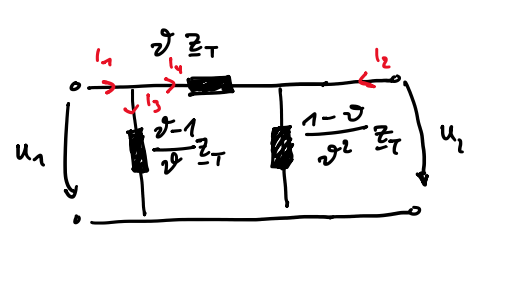
\includegraphics[width=.7\textwidth]{fundamentals/pi_transformer.png}
    \caption[$\Pi$-representative circuit of a transformer with a longitudinal tap changer]{$\Pi$-representative circuit of a transformer with a longitudinal tap changer; own figure after \autocite{machowskiPowerSystemDynamics2020,burlakinEnhancedVoltageControl2024}}
    \label{fig:pi-transformer}
\end{figure}

\begin{align}
    \underline{I}&=\underline{\mab{Y}} \cdot \underline{U} \notag \\[12pt]
    \begin{bmatrix}
        \underline{I}_1 \\
        \underline{I}_2
    \end{bmatrix}&= 
    \begin{bmatrix}
        \underline{Y}_{11} & \underline{Y}_{12} \\
        \underline{Y}_{21} & \underline{Y}_{22}
    \end{bmatrix} \cdot
    \begin{bmatrix}
        \underline{U}_1 \\
        \underline{U}_2
    \end{bmatrix} \label{eq:admittance}
\end{align}

The admittance matrix of a two port network can be expressed after \textcite{machowskiPowerSystemDynamics2020} as \autoref{eq:admittance}. For the $\Pi$-model of an \acs{OLTC} transformer it is leading to \autoref{eq:admittance-oltc}.
% \sidenote(1.7cm){$\Pi$-admittance matrix}
\begin{align}
    \underline{\mab{Y}}_\mathrm{\Pi,T}&= 
    \begin{bmatrix}
        \underline{Y}_\mathrm{T} & -\underline{\vartheta}\underline{Y}_\mathrm{T} \\
        \underline{\vartheta}^*\underline{Y}_\mathrm{T} & -\underline{\vartheta}^*\underline{\vartheta}\underline{Y}_\mathrm{T}
    \end{bmatrix} \label{eq:admittance-oltc}
\end{align}
Another way of writing down the admittance matrix is shown in \autoref{eq:admittance-oltc-2}. It is considering, that the matrix can be split up in a symmetric, constant part, and a variable current injection part. The latter is not symmetrical and depends on the tap position of the transformer. Therefore in some simulation algorithms the static part is used in the admittance matrix, and the variable part is considered in the current injection vector. \autocite{machowskiPowerSystemDynamics2020}

\begin{align}
    \begin{bmatrix}
        \underline{I}_1 \\
        -\underline{I}_2
    \end{bmatrix} &=
    \begin{bmatrix}
        \underline{Y}_\mathrm{T} & -\underline{Y}_\mathrm{T} \\
        -\underline{Y}_\mathrm{T} & \underline{Y}_\mathrm{T}
    \end{bmatrix}
    \begin{bmatrix}
        \underline{U}_1 \\
        \underline{U}_2
    \end{bmatrix} -
    \begin{bmatrix}
        \Delta \underline{I}_1 \\
        \Delta \underline{I}_2
    \end{bmatrix}\text{, where } \notag \\[12pt]
    \begin{bmatrix}
        \Delta \underline{I}_1 \\
        \Delta \underline{I}_2
    \end{bmatrix} &=
    \begin{bmatrix}
        \underline{0} & (\underline{\vartheta}-1)\underline{Y}_\mathrm{T} \\
        -(\underline{\vartheta}^*+1)\underline{Y}_\mathrm{T} & (\underline{\vartheta}^*\underline{\vartheta}+1)\underline{Y}_\mathrm{T}
    \end{bmatrix}
    \begin{bmatrix}
        \underline{U}_1 \\
        \underline{U}_2
    \end{bmatrix} \text{ leading to } \notag \\[12pt]
    \underline{\mab{Y}}_\mathrm{\Pi,T}&= 
    \begin{bmatrix}
        \underline{Y}_\mathrm{T} & -\underline{Y}_\mathrm{T} \\
        -\underline{Y}_\mathrm{T} & \underline{Y}_\mathrm{T}
    \end{bmatrix} -
    \begin{bmatrix}
        \underline{0} & (\underline{\vartheta}-1)\underline{Y}_\mathrm{T} \\
        -(\underline{\vartheta}^*+1)\underline{Y}_\mathrm{T} & (\underline{\vartheta}^*\underline{\vartheta}+1)\underline{Y}_\mathrm{T}
    \end{bmatrix} \label{eq:admittance-oltc-2}
\end{align}

\subsubsection*{Per unit system specialities}

Reactances and resistances are referred to the base voltage and apparent power of the operational unit, such as the transformer. The power system simulation uses its own base voltage and base apparent power, enabling the use of one single calculation domain. This is done to simplify the calculation and to make the results easily comparable to each other. Hence, the reffered values have to be transformed from the equipment based values to the simulation based values. The relations and conversions are defined as follows.

\begin{align}
    &\underline{Y}_\mathrm{T}=\frac{1}{r_\mathrm{T} + x_\mathrm{T} \cdot j} \cdot \frac{b_\mathrm{T} \cdot j}{2} \notag \\[12pt]
    &\underline{Y}_\mathrm{T,~sim}=\underline{Y}_\mathrm{T} \cdot \frac{S_\mathrm{n}}{S_\mathrm{n,~sim}} \label{eq:y-t-based} \\[12pt]
    &\underline{U}_\mathrm{whatever,~sim}=\underline{U}_\mathrm{whatever} \cdot \frac{S_\mathrm{n}}{S_\mathrm{n,~sim}} \label{eq:voltages-based}
\end{align}

Displayed like in \autoref{eq:y-t-based}, the characteristic of the operational unit is referred to the simulation base value. Here, the admittance of the transformer is multiplied with its own rated apparent power, then devided by the apparent power of the simulation system. Similar, the voltages are calculated via \autoref{eq:voltages-based}. This specialities are considered in the tap changer modeling, thus further information is given in \autocite{machowskiPowerSystemDynamics2020}, Appendix A.

\commenting{
    Additionally to consider:
    \begin{itemize}
        \item D-q transformations (???),
        \item Frequency domains: reactances and inductances are dependent and can change with the base frequency,
        \item Torque and power relations.
    \end{itemize}
    }

\subsection{Open-Source Power System Simulation tools}
    
\commenting{
    Some information about other open source python power system simulation tools, such as:
    \begin{itemize}
        \item Pandapower,
        \item TOPS,
        \item ... .
    \end{itemize}
    Build up like a scan (see Georg's thesis).
    
    BUT: As well including the there used implementation of transformers mathematical background and complexity.
}
        
%%%%%%%%%%%%%%%%%%%%%%%%%%%%%%%
\section{Voltage stability basics}

\subsection{Voltage stability definitions, classifications, and conditions}
A Practical introduction to voltage stability assessment, methods and indices is given in the standard and extending literature of \textcite{rueda-torresEvaluationVoltageStability2024,danishVoltageStabilityElectric2015,cutsemVoltageStabilityElectric1998}.

\commenting{
    Interesting to note/implement here: Basic classification, definitions, and the nature or conditions of voltage stability. Such as
    \begin{itemize}
        \item Short term vs. long term
        \item Static vs. dynamic
        \item Transmission driven vs. load driven vs. generation driven; stability/instability, and/or contributions 
        \item Influence OLTC: Restoring voltage level, but not adding reactive capacities; hence adding risk of voltage collapses
        \item Load vs. transmission aspects
        \item Example mechanism: \textbf{Collapse effect of the nordic test system} \autocite{vancutsemTestSystemsVoltage2020,cutsemVoltageStabilityElectric1998}
    \end{itemize}
}
        
\begin{table}
    \centering
    \caption{Voltage instability types and different time frames with examples; after \quelle}
    \small
    \renewcommand\tabularxcolumn[1]{m{#1}}
    \vspace*{12pt}
    \begin{tabularx}{\textwidth}{llXX}
        \toprule
        \textbf{No} & \textbf{Type} & \textbf{Cause of incident} & \textbf{Time frames} \\
        \toprule
        1 & Long-term & Slowly use up of reactive reserves and no outage & Several minutes to several hours \\
        2 & Classical & Key outage leads to reactive power shortage & One to five minutes \\
        3 & Short-term & Induction motor stalling leads to reactive power shortage & Five to fifteen seconds \\
        \bottomrule
    \end{tabularx}
\end{table}

\subsection{Stability Indices}

One easy idea for obtaining a stable operation is looking at the Jacobian Matrix. If this matrix is getting singular, the System will not remain in a stable operation. Singularity of matrices is checked by follwing two hypothesis tests:
\begin{align}
    &\det(\mab{J})=0 \label{eq:jacobian-det} \\[12pt]
    &J \times J^{-1} \uparrow \label{eq:jacobian-rank}
\end{align}
The Jacobian Matrix is defined as:
% \sidenote(5.2cm){Jacobian Matrix}
\begin{align}
    \mab{J}=
    \begin{bmatrix}
        \Delta \mab{P} \\
        \Delta \mab{Q}
    \end{bmatrix}&=
    \begin{bNiceArray}{c|c}
        \mab{H} & \mab{M'} \\ \hline
        \mab{N} & \mab{K'}
    \end{bNiceArray} \cdot
    \begin{bmatrix}
        \Delta \delta \\
        \Delta V/V
    \end{bmatrix} \notag \\[12pt]
    \begin{bmatrix}
        \Delta P_1 \\
        \vdots \\
        \Delta P_n \\ \hline
        \Delta Q_1 \\
        \vdots \\
        \Delta Q_n
    \end{bmatrix}&=
    \begin{bNiceArray}{ccc|ccc}
        \frac{\partial P_1}{\partial \delta_1} & \hdots & \frac{\partial P_1}{\partial \delta_n} & V_1\frac{\partial P_1}{\partial V_1} & \hdots & V_n\frac{\partial P_1}{\partial V_n} \\
        \vdots & \ddots & \vdots & \vdots & \ddots & \vdots \\
        \frac{\partial P_n}{\partial \delta_1} & \hdots & \frac{\partial P_n}{\partial \delta_n} & V_1\frac{\partial P_n}{\partial V_1} & \hdots & V_n\frac{\partial P_n}{\partial V_n} \\ \hline
        \frac{\partial Q_1}{\partial \delta_1} & \hdots & \frac{\partial Q_1}{\partial \delta_n} & V_1\frac{\partial Q_1}{\partial V_1} & \hdots & V_n\frac{\partial Q_1}{\partial V_n} \\
        \vdots & \ddots & \vdots & \vdots & \ddots & \vdots \\
        \frac{\partial Q_n}{\partial \delta_1} & \hdots & \frac{\partial Q_n}{\partial \delta_n} & V_1\frac{\partial Q_n}{\partial V_1} & \hdots & V_n\frac{\partial Q_n}{\partial V_n} \\
    \end{bNiceArray} \cdot
    \begin{bmatrix}
        \Delta \delta_1 \\
        \vdots \\
        \Delta \delta_n \\ \hline
        \Delta V_1/V_1 \\
        \vdots \\
        \Delta V_n/V_n
    \end{bmatrix}
\end{align}

Although this method seems easy to implement, there are some numerical problems realted to that. Checking if a Matrix is singular with numerical mathods, can only be realised as a probablilty expression. A result could be, that the determinant of the matrix is below a certain threshold. The algorithm would propose, that the matrix is probabilistic singular. \commenting{[QUELLE]} This problem leads to the necessity of applying other methods or indices for stability assessment. \textcite{danishVoltageStabilityElectric2015} is proposing a few other indices, that are based on the Jacobian Matrix, and shows comparitive characteristics between Jacobian Matrix and system variable based voltage stability indices. These Jacobian Matrix based indices are listed and further described in \autoref{app:jacobian-voltage-indices}, while the comparative characteristics are described in \autoref{app:jacobian-vs-system-indices}. 

\subsection{Assessment methods}
        
\subsection{Analytical stability calculation of static power systems}
        
%%%%%%%%%%%%%%%%%%%%%%%%%%%%%%%
\section{Control engineering theory}

\subsection{Commonly used on-load tap changer control}

A few basics are in the interest, understanding differences between real world beahavior, or possible ways of building up a \acs{OLTC} transformer control. This control theory difference can be limiting as well for the results and objectives compared to the actual possible control in the field.

\subsubsection{Typical presets are manually set}

The target voltage is typically set from the control room of the grid operator, coming from pre-calculated load flow analysis. This can be set hours before, or even day-ahead with the estimated loads of the grid. This value is set locally for each operating unit subsequently. The control is then operating locally and without further involvement of the grid operator. \quelle

\subsubsection{Discrete controllers are used in the field}

Typically the used controller in the field is a discrete controller, which can change tap positions under load within a time frame of around few seconds. Practical tap steps are around $2~\mathrm{\%}$ of the overall transforming ratio. The control is set up with a dead band, to avoid unnecessary tap changes. It is necessecary to note here, that this control and its mathematical caracteristics contains logical elements, blocks, and delays, which cannot be translated in a typical control theory transmission function. This leads to the missing possibility to easily obtain mathematical stability for the control of the overall considered power system. \quelle

\subsection{Dynamic voltage stability}

\commenting{
    Can I really express this as \glqq Controller theory\grqq?
}

\subsection{Bifurcations and Chaos theory control}

\commenting{
    Is this necessary or already out of scope?
    \begin{enumerate}
        \item Fuzzy Control mechanisms,
        \item Neural Networks,
        \item Bifurcations.
\end{enumerate}
}
%!TEX root = ../main.tex

%%%%%%%%%%%%%%%%%%%%%%%%%%%%%%%
%%%%%%%%%%%%%%%%%%%%%%%%%%%%%%%
\chapter{Methodical Modeling}
\label{chap:methodical-modeling}

\begin{textblock*}{.7\textwidth}(70mm-\offset,25mm-\offset)
        \begin{fquote}[Albert Einstein]
            All models are wrong, but some are useful.
        \end{fquote}
\end{textblock*}

This chapter mehodical modeling focusses on the description of thoughs and structures of the implementation in Python.
It is not evolving more than necessary details about the package {\itshape diffpssi}, but trying to comprehensible illustrate the structure of the algorithms theirselves and the necessaary bordering interfaces.

%%%%%%%%%%%%%%%%%%%%%%%%%%%%%%%
%%%%%%%%%%%%%%%%%%%%%%%%%%%%%%%
\section{Transformer Equipment Modeling}
\label{sec:transformer-modeling}

This section respectively focusses on the dynamics and model behavior of the transformer itself.
It is split according to the structure of the implementation itself, into the modeling of the $\Pi$-model and the tap changer control.
For the last mentioned, there are different control schemes implemented and thus described in the subsequent section.
In the beginning, the rough software structure idea of the extension is described, continuing with a dive into the mathematical relations, and specialities.  

%%%%%%%%%%%%%%%%%%%%%%%%%%%%%%%
\subsection{Software Architecture Design}
\label{sec:modeling-architecture}

The first scope of the \textit{diffpssi} extension is to form a modular and easy to maintain class structure. 
The background is to enable support of adding other types of transformers and resp. or connected control circuits.
A conceptual chart of this architecture is shown in \autoref{fig:transformer-architecture}.
It is representing only necessary packages, classes, and and attributes for the transformer and its control.

\begin{figure}[htbp!]
        \centering
        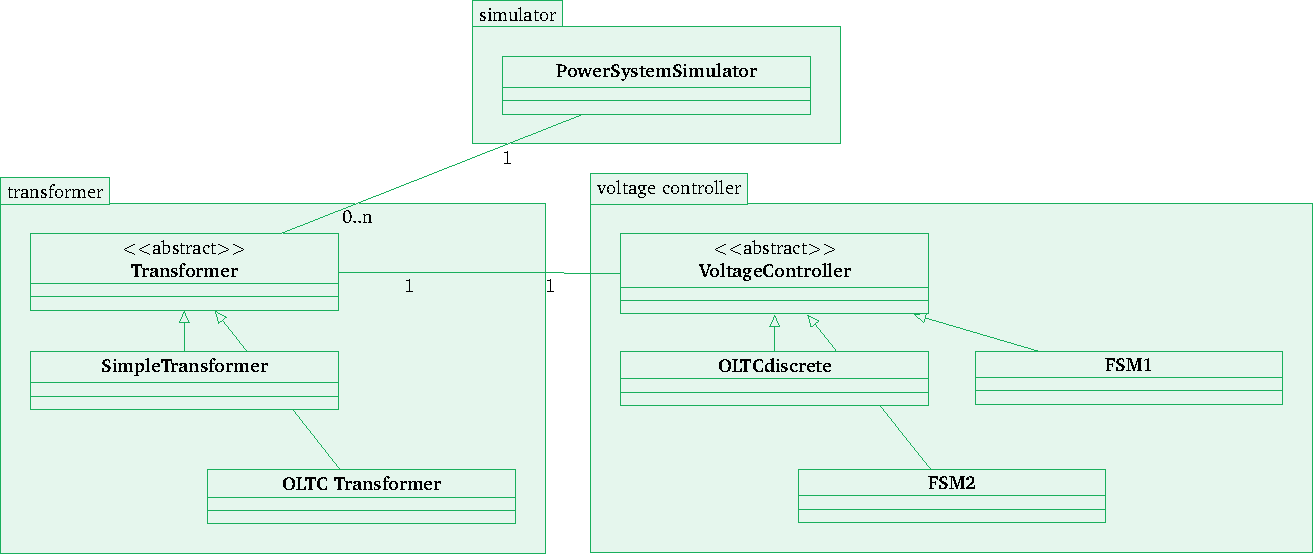
\includegraphics[angle=90, height=18cm]{./tikz_graphics/images/software_structure.pdf}%{modeling/diffpssi_trafo_architecture.png}
        \caption[Architecture of the implemented models in \textit{diffpssi}]{Architecture of the implemented models in \textit{diffpssi}; Using abstract classes for correct interfaces and improved reusability; only necessary packages, modules and classes are depicted}
        \label{fig:transformer-architecture}
\end{figure}

The main class for the Power System Simulation, hosting the central data structures and results is called \textit{PowerSystemSimulator}.
Models, busses, lines, but also transformer objects are connected to each other, and on top of that referenced in the main simulation object as groups represented by lists.
The transformers shall be connected in the same way as before, but differing from the old transformer considering just the serial impedance, a simple non-tapping transformer sall be integrated next to a longitudinal tap-changing one.
The room for possible extension, meaning phase shifters or mixtures of these models can be kept by using a abstract class as interface.
This forces the inheritating classses to override the necessary methods, have at least the mandatory attributes.
Copying existing and functional structures is easier as well.

The transformer itself is just a mathematical representation of the pi model, considering a serial impedance and two shunt branches.
Connected control units shall be excluded from this, to ensure modularity as well. 
Therefore a lot of different control tweaks can be easily implemented and tested.
To provide a consistant interface here as well, the abstract class \textit{Voltage$\_$Controller} is used.
Within this thesis implemented are a discrete and a continuous \acs{OLTC} controller, and two discrete \acs{FSM} controllers.
These reference to the standardized control blocks as well, e.g. PT1 or Integrating elements.

%%%%%%%%%%%%%%%%%%%%%%%%%%%%%%%
\subsection{Implementing a \texorpdfstring{$\Pi{}$}{}-Representative Circuit with Variable Ratio}

Before detailing in the software side of the implemetation, some mathematical differences are explained.
This results on the one hand from the major differences in the standard literature, especially between \textcite{machowski_2020} and \textcite{kundur_2022}, resp. \textcite{milano_2010}.
On the other hand, these differences occur as well in the comparative and validation simulation software \textit{DIgSILENT PowerFactory}.
The use of these different models is described in its technical reference manual \quelle. 

%%%%%%%%%%%%%%%%%%%%%%%%%%%%%%%
\subsubsection{Mathematical Description and Definitions}

\sidenote{Important definitions and literature differences}
Firstly it is important to comment on the use of indices in this thesis, and especially following for this chapter.
The index 1 is always referring to the \acs{LV} side, the index 2 to the \acs{HV} side. 
The impedances can be concentrated and related to either the \acs{LV}, or as usual to the \acs{HV} side of the transformer. 
The in \autoref{sec:trafo-model} used derivation is using a relation on the \acs{HV} side.
The same accounts for the definition of the \acs{OLTC} ratio $\underline{\vartheta}$.     
The \acs{OLTC} ratio $\underline{\vartheta}$ in this thesis is always placed on the HV side.
% If one wants to place this ratio on the \acs{LV} side, the in this thesis defined ratio has to be used reciprocal.
% For the simulation tool, this is crucial to understand and define correctly in order to acquire correct results.

\sidenote{Definition OLTC ratio}
This thesis focusses on an ideal tap changer model at first, other possible considerations from \autoref{sec:further-considerations} are neglected.
As vector groups are as well not considered, the tap ratio stays solely a rational number.
Like previously mentioned, and consequently described, the ratio $\vartheta$ is then placed on the \acs{HV} side of the transformer.
The \acs{OLTC} ratio $\vartheta$ is then defined as:
\begin{align}
        \vartheta_\mathrm{HV} &= 1 + k \cdot \Delta v \label{eq:tap-ratio-hv} \\[6pt]
        \text{with } k &\in [k_\mathrm{min};k_\mathrm{max}]; k_\mathrm{min} \equiv  -k_\mathrm{max} \label{eq:tap-pos}
\end{align}
Within this definition, $k_\mathrm{min}$ defines the minimum tap position, $k_\mathrm{max}$ the maximum \acs{OLTC} position. 
The variable $\Delta v$ defines the change of the ratio in percent for alterning one position.

% \sidenote{Representation of\\Vector Groups}
% Voltage angle shifting through the influence of vector groups, meaning a different wiring and thus magnetic coupling of the transformer can be expressed within the transformer model. 
% By mathematically applying a turning vector with the length of one to the overall tap ratio, this can be included in the model. 
% Mathematical, this is expressed by the following equation. 
% The characteristic number $n_\mathrm{T}$ is relating to to angle, with one step being equal to $30^\circ$ angle ratio.
% \begin{align}
%         \underline{a}_\mathrm{T} &= \exp(j \cdot n_\mathrm{T} \cdot \frac{\pi}{6}) \label{eq:vector-group}
% \end{align}

\subsubsection{Mathematical Different Representations}

\sidenote{Relation to the LV side}\mycomment[MK]{Rewrite this section to just Machowski style and its difference -> less confusion}
When one either wants to relate the transformer admittance, or the tap ratio to the \acs{LV} side, a different admittance matrix definition has to be used.
The admittance matrix is then defined as:
\begin{align}
        \underline{\mab{Y}}_\mathrm{\Pi,T}&= 
        \begin{bmatrix}
            \underline{Y}_\mathrm{T} & -\underline{\vartheta}\underline{Y}_\mathrm{T} \\
            \underline{\vartheta}^*\underline{Y}_\mathrm{T} & -\underline{\vartheta}^*\underline{\vartheta}\underline{Y}_\mathrm{T}
        \end{bmatrix} \label{eq:admittance-oltc}
    \end{align}
The following mathematical result leads to a necessary change in the software implementation.
Either \mycomment[MK]{Is this actually the case? Or is it a different condition?}
\begin{itemize}
        \item the admittance matrix bus indices have to be changed,
        \item the tap ratio has to be reciprocal according to \autoref{eq:tap-ratio-lv}, or
        \item using the \acs{HV} side admittance matrix, but changing the tap ratio definition and the bus indices.
\end{itemize}
These different ways of variable and placing definitions also characterize the ways, the admittance matrix of the \acs{OLTC} transformer is derived from either \textcite{machowski_2020}, versus \textcite{kundur_2022}, \textcite{milano_2010}, or \textcite{burlakin_2024}.
Another thought or way of representing a transformer with off-nominal ratio is described in the appended \autoref{app:current-injection-model}.
\begin{align}
        \vartheta_\mathrm{LV} &= \frac{1}{1 + k \cdot \Delta v} \label{eq:tap-ratio-lv}
\end{align}

\subsubsection{Design and Implementation of Algorithmics}

\sidenote{Necessary methods}
As afore described in the general architecture of the extension, interfacial methods and attributes are implemented.
Starting with the necessary methods, which can be devided into expectations from the framework itself, the operational unit type transformer, and the novel consideration as dynamic model.
From the framework itself, mainly the three methods \textit{initialize()}, \textit{enable$\_$parallel$\_$simulation()}, and \textit{get$\_$value()} are included.
All submodels have to be initialized with the preset of the measurement voltage at the to be measured bus. 
This accounts only for the \acs{OLTC} related transformers, all others pass this functionality.
To enable parallel simulations, all attributes have to be set as tensors in the expected format of the simualtions.
This is achieved trough multiplying the value with a tensor of the shape $(1, {parallel\_sims})$.
For accessing additional, or partly calculated values of interest in the model, the last method is computed.
Although this is currently also an empty function, it can be extended and called by the recorder function of the simulation framework.

Necessary methods from the transformer unit type are the calculation of the static and the dynamic admittance matrix.
As for the transformer, and the current goal of implementation, both methods are identical.
If one would want to implement also an automatic tap position configuration for load flow solving, this would provide the sufficient interface.
In the method \textit{calc$\_$admittance()}, the afore described transformer admittance matrix is calculated and inserted into the system admittance matrix at each time step.
In the begining of the \acs{OLTC} transformer, the current measurement bus voltage is aquired and handed to the output function of the connected voltage controller.
This output function is giving back the transformer ratio dependent on the current bus voltage. 
The transformer ratio is the set as an attribute and the admittance then can be calculated and updated.
As an initial value for performing load flow analysis, this ratio is set to $1$ p.u.

In order to consider this model as dynamic, three methods have to be implemented in the transformer itself: \textit{differential()}, \textit{get$\_$state$\_$vector()}, and \textit{set$\_$state$\_$vector()}.
As the transformer itself is containing no dynamics, buit its connected controllers are, these methods solely call the methods in the controllers accordingly.

\sidenote{Necessary attributes}
The necessary attributes of the transformers alowing the functions to work properly are implemented as following.
The admittance matrix is always also set as attribute.
This allows for evaluation and mapping through the recorder function.
Every transformer has a name, a resistance, a reactance and a susceptance attribute, as well as the transformer ratio $u$, resp. $u_\mathrm{l}$ for the solely longitudinal part.
For the vector group angle rotation, the attribute theta is added.
Additionally, the mandatory system related variables for the system base apparent power, the transformer apparent power, the voltages at both busses, and the parallel simulations are necessary.
Considering the direction of the transformer in the system, the set of variables declaring the bus name, id, and voltage of the \glqq from\grqq~bus is partly defining the installation.
On top of these, tap side and the measurement bus are completing the clear identification.

\sidenote{Comments on the installation}
Focussing more on the installation direction, following procedure is applied in the calculation of the admittance matrix, as it is handed over to the simulation just as tensor.
A dictionary would be possible as well, as it would possible to namely declare the tap side and non tap side index resp. impedance.
As used attributes, the attribute \textit{from$\_$bus} and \textit{tap$\_$side} receive either the flag \textit{hv} or \textit{lv}.
For the later attribute the allocation is in the responsibiliity of the user, the first one is allocated through checking the voltages of the busses.
If the \textit{from$\_$bus} is the lower value of the voltages, the value \textit{lv} is assigned, and other way round.
The admittance is then calculated for the base scenario, if the tap side of the transformer is not the from bus.
For this scenario \autoref{eq:admittance-matrix-pi} is used.
If the values match, then the admittance matrix indices are switched, and the admittance matric is set as
\begin{align}
        \underline{\mab{Y}}_\mathrm{\Pi,T}&=\underline{Y}_\mathrm{T} \cdot
        \begin{bmatrix}
                \frac{1}{\underline{\vartheta}\underline{\vartheta}^*} & -\frac{1}{\underline{\vartheta}^*} \\
                -\frac{1}{\underline{\vartheta}} & 1
        \end{bmatrix}. \notag
\end{align}

% \sidenote{Aditional considerations}
% \commenting{
%         Additionally interesting extensions:
%         \begin{itemize}[nosep]
%                 \item In which direction the matrix has to be inserted?
%                 \item Transformer types
%                 \item Measurement side detection for interface towards Tap changer control
%         \end{itemize}
% }


%%%%%%%%%%%%%%%%%%%%%%%%%%%%%%%
\subsection{Tap Changer Control Modeling}
\label{sec:modeling-tap-changer-control}

\sidenote{General interface structure}
As the tap changers, or voltage controllers for the longitudinal ratio of an \acs{OLTC}, are solely controllers, and therefore can also be dissembled in just control blocks, the necessary methods for integration in the module \textit{diffpssi} are limited.
Therefore the abstract base class, used as an interface class here, is containing the funtions \textit{differential()}, \textit{get$\_$state$\_$vector()}, \textit{set$\_$state$\_$vector()}, and \textit{get$\_$output()} for the control purposes.
Adiitionally, as every other dynamic class, both methods \textit{initialize()} and \textit{enable$\_$parallel$\_$simulation()} are included in the same way as described before as well.
In case it is needed, every controller is specifying the function \textit{update$\_$vref()}, to update the reference voltage of the control. 
The only varied standard method is \textit{get$\_$output()}, but additional needed ones are necessary dependent on the controller.
These methods are detailed in the subsequent parts of this subsection.

\sidenote{Deadband block}
Before going deeper into the control loops, two basic control blocks are implemented into the framework.
The first one is the realization of a deadband block.
This means that if the input value is smaller than a defined threshold, the output will be zero, otherwise it is returning the input value.
The differential function for this block is not necessary, as it is just reacting on the imput and not building up any dynamics or relations towards previous inputs.
The only necessary concern is the enabling of parallel simulations as well, to stay consistent with data types in the calcualtion.

\sidenote{Integrator block}
The second implementated basic block is an integrator, commonly knwon as I-block in control engineering.
This block has got relations to previous inputs and therefore a differential function, as well as methods for setting and reading the state vector.
This attribute is a storage for the state in the previous timestep, with the differential the next state can be calucated.
As the method \textit{get$\_$output()} is only called by the models, this is the connection to input variables.
An attribute input is set to the handed over value from that function, enabling the differential to be calculated.
Additionally, the output is set to the current state of the control block times a constant multiplication factor $k_\mathrm{i}$ of the integrator.
This integrator is extended by the possibility to set an limiter, as well to externally reset the state and the input variables of the object.
The differential function for an integrator is the input variable times the time step.
As this multiplication is done in the solver function of \textit{diffpssi}, the return of te differential is solely the input value.
The last part is the initialization process, where the first output of this block has to be set, meaning setting the current initial state as the wished or needed output devided through the mulatiplication factor $k_\mathrm{i}$.
This first output is then also returned.

\subsubsection{Discrete Control Loop}

\sidenote{General aspects\\and references}
This control method represents the currently most used and thus representative control scheme for \acsp{OLTC}. 
With the mechanic nature of the switching mechanism, the control loop can only access discrete ratios within time frames of around a few seconds. 
Such a discrete control loop is described by \textcite{milano_2011,milano_2010}. 
A scheme of this control loop is shown in \autoref{fig:discrete-control-loop}.
This control loop type is beneficial due to its accurate representability of current \acs{OLTC} abilities. 

\begin{figure}[htbp!]
        \centering
        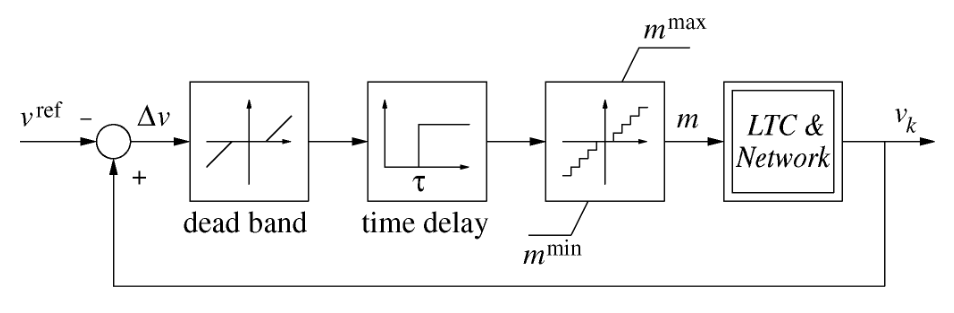
\includegraphics[width=\linewidth]{modeling/oltc_control_scheme.png}
        \caption{Discrete control loop of an \acs{OLTC}; from \textcite{milano_2011}}
        \label{fig:discrete-control-loop}
\end{figure}

\sidenote{get$\_$output()}
\commenting{
        The controller is actively changing the algebraic funtions of the simulation environment, therefore it is quasi dynamic. 
        The controller output logic is called, when updating the admittance matrix of the transformer. 
        Additionally, the differential functions of the connected simple controllers, like integrators, PT1-blocks, etc., are called by the solver and are thus part of the differential equations. 
        The logic determines the physical interpretation of the \acs{OLTC}, and therefore
        \begin{enumerate}
                \item If the OLTC has to switch,
                \item When the switching operation is finished, and
                \item What the current, or in case after a switching the new, tap ratio is.
        \end{enumerate}
        It is important to note, that this structure relies on the calculation of the dynamic admittance matrix on each time step.
}

\sidenote{switching()}
The only additional method for the discrete standard \acs{OLTC} scheme is called \textit{switching()}.


\commenting{
        \begin{itemize}[nosep]
                \item Control scheme
                \item Switching logic and behavior (voltage tracking)
                \item 
                % \item How to automatically determine switching direction?\\
                % -> switching direction dependent on what? (load-flow direction?)
                % \item Controller set points: also dependent on load flow?
                % \item How can I change the transformer control setpoints to be load flow dependent?
        \end{itemize}
}

% \lstinputlisting[caption={Output Function of the discrete OLTC controller 2},captionpos=b,style=style-python,label=lst:oltc-discrete2]{images/code/oltc-discrete.py}

% \subsubsection{Continous Control Loop}

% \commenting{Just describe the difference to the discrete \acs{OLTC}. Probably just the function get output is different, as all supplementary and attributes stay identical.}

% The implementation of an continous control scheme ia fairly straight forward.
% The desired continous block is a PT1 element with a limiter, which is already implemeted in the python module \textit{diffpssi}.
% All function say as they are descibed in the previous discrete \acs{OLTC} controller, altough the method \textit{switching()} is not needed and thus removed.
% The PT1 element is initialized with a user specified time constant, and the \acs{OLTC} tap ratio boundaries as limits.
% Additionally an error bandwith is defined for eliminating numerical noises.
% This is set to $0.01$.
% The voltage difference is then calculated, but not directly handed over to the PT1 function.
% The input to control with the PT1 is calculated by the reference voltage added to a impact factor times the voltage difference \autocite{milano_2010}.
% Typically this is three times the error, or difference.
% This cannot be realized through the gain of the PT1 block, as it would account for the complete sum.


\subsubsection{Control Schemes for the Fast Switching module}

\commenting{\textbf{ATTENTION:} Two models availabel, described in the paper, where the FSM is preferred and the 'novel' scheme where usage of FSM or OLTC ios dependent on the tap skipping and the deas band. Only the last is usable for verification!}

\commenting{
        \begin{itemize}[nosep]
                \item Describe implementation
                \item Describe benefits / drawbacks
                \item Control scheme
                \item Switching logic and behavior (voltage tracking)
        \end{itemize}

        No restrictions implemented for theta max or min! Solely limited through the max positions.
}

\sidenote{Functional basics\\of a FSM}
Describe the operational logic and structure of the \acf{FSM} first.

\sidenote{Control logic}
A control logic for a so called \acs{FSM} has been presented from \textcite{burlakin_2024}, and illustrated in \autoref{fig:fsm-control-loop}.

\sidenote{Implementation\\differences}
However, the implementation logic in Python is slightly differing from the presented scheme in \autocite{burlakin_2024}, simply for not overcomplication of the code and therefeore debugging. 
The implementation is similar to the afore discussed one of a standard \acs{OLTC} controller. 

\sidenote{Differences of variations}

\subsubsection{Characterization of the Implemented Control Schemes}
% \sidenote{Characterization\\and validation}

For characterization of the control output, two different approaches are selected.
First, a step or jump function is applied, for a maximum gradient inspection.
Further, a continous function is selected, incrementing the voltage difference on the control loop.
This could be exponential, exponential decaying, or something like linear increasing as scenario in the middle.
As the tap changer has maximum positions, and therefore also a operational band, the exponential decaying function is selected as second characterizing input.

\begin{figure}[htbp!]
        \centering
        \includegraphics[width=.7\linewidth]{development_files/validation/data/oltc_control_characterization.pdf}
        \caption[Characterization of the OLTC control loops]{Characterization of the OLTC control loop; the input function simulates the to be regulated voltage, the output functions are characterized by $o(t)=i(t) \cdot \underline{\vartheta}_\mathrm{trafo}$}
        \label{fig:oltc-control-characterization}
\end{figure}

%%%%%%%%%%%%%%%%%%%%%%%%%%%%%%%
\subsection{Experimental: Extended Ideas and Improvements}
\label{sec:experimental-modeling}

This subsection introduces a few ideas for improvements of the \acs{FSM} voltage controller.
As this is based on observations during the development, validation or analyzing case studies, one might consider going through this after understanding the thoughts of the other remaining parts.
Doing a re-read at the end would be beneficial either way.   

\subsubsection{Operational Oriented FSM Control}

\ai{
        The time constants are used in the control model to model the influnce of switching operation duration.
        This is coming from the mechanical movement of the OLTC, therefore it is the \glqq maximum possible dynamic behavior\grqq.
        The FSM doesnt't have this limitation, as it can switch after every $\sin$ period (0.02 s).
        
        Currently we can access two different operational modes: Prefer the FSM, or switching on how far is the voltage deviated in both time constants.
        This is a first, more targeted approach towards concerning dynamics in the voltage behavior, but still based on the time constants, not only limited through them.
        
        Why don't we approach a control strategy, which is only considering dynamics, and let the time constants just restrain and block the switching.
        Meaning, that the faster the voltage deviates, the more the FSM gets preferred, the slower the dynamics, the more the standard OLTC gets preferred.
        This could also lead to neglecting a dead-band, and still preventing so called tap-hunting.

        Combined with an operational oriented thought, keeping the possible switching movements of the FSM at its maximum / optimal position.
        This would mean, that in more static times, the FSM switches in its defined \glqq as neutral defined\grqq position and the OLTC is balancing the devaitions.
        One might call this a corrective supervision or monitoring.
}

\subsubsection{Alternative Tap Skipping Logic}

\ai{
        Curretnly the tap skipping logic is formulated as
        \begin{quote} \itshape
                How many times does the deadband fit into the voltage deviation?
        \end{quote}
        to determine the floored number of skips (with contraints). 
        Meaning in mathematical terms: 
        \begin{align}
                \eta(t)=\text{floor}\bigg(\frac{\vert \Delta v(t)\vert}{db_\mathrm{v} \cdot \Delta m}\bigg)
        \end{align}

        An alternative approach would be: 
        \begin{quote} \itshape
                How many switches of the FSM would the current offset voltage bring back to the reference value?
                How many times does one FSM switch fit into the voltage deviation?
        \end{quote}
        Meaning in mathematical terms:
        \begin{align}
                \eta(t)=\text{floor}\bigg(\frac{\vert \Delta v(t)\vert}{\Delta k \cdot \Delta m}\bigg)
        \end{align}
        
        Last approach should be more accurate for different pairs of preset values (deadband, added voltage per tap, etc.).
        BUT: both approaches do not consider the true effect on the dynamic loads and the grid.
        Different grid strengths could react differently on the applied transformer ratio.
}

\subsubsection{Varying the Voltage Setpoint and Target Calculation}

\commenting{
        Here, another idea of control target creation shall be mentioned. 
        Instead of a fixed bus voltage reference, the difference of both bus voltages is considered. 
        Further, the sign of that difference is used to determine the direction of the tap change.
}

\ai{
        Different things to consider here:
        \begin{itemize}
                \item \textbf{Load-flow Direction} with ranking the bus voltages in p.u. against each other,
                \item \textbf{Dynamic Setpoints} through automated calculation of target voltage (nose curves),
                \item \textbf{Different Control Input} as not with a fixed target value, but the difference between both bus voltages; thus tentiative, becuase it is not considering supporting the load, but falsly trying to prevent a wrong switching direction.
        \end{itemize}
}


%%%%%%%%%%%%%%%%%%%%%%%%%%%%%%%
%%%%%%%%%%%%%%%%%%%%%%%%%%%%%%%
\section{Application of Voltage Stability}
\label{sec:application-voltage-stability}

As previously discussed in the fundamentals of voltage stability, \autoref{sec:voltage-stability}, ensuring power quality is a secondary goal.
Concerning that voltage stability, regardless of short- or long-time evaluation, is a topic of power quality, it is hard to determine stability or instability.
In terms of static possible solutions, there are a lot of tools determing the critical points, as well as the current distance to it.
Looking into the short-term, more dynamic assessment, there are less elegant solutions. 
This thesis is trying to keep the perspective on both, short- and long term voltage stability.
The following is the approach to synthesize a toolset for voltage stability analysis, that is at least dynamically comparable.
As nose curves are a valid and popular tool, they shall be implemented first. 
Afterwards the time series calculation is tried to integrate into this static evaluation, including tap changer dependent behavior.
Lastly, a more dynamic rating of a sceario shall be computed, enabling also the confirmity with grid codes for example.

%%%%%%%%%%%%%%%%%%%%%%%%%%%%%%%
\subsection{Generation of Nose Curves}
\label{sec:nose-curves}

This section describes the implementation of a prevoiusly discussed static voltage analysis tool.
The generation of nose curves helps in finding the critical loading of the system at the bus of interest, although it is static nature. 

\subsubsection{Basic Simplification Idea}

\textcite{ajjarapu_1992, ajjarapu_2007} are presenting a method for numerical calculation of nose curves in their work. 
It is called {\itshape Continuation Power Flow} and is based on a modified Newton-Raphson method.
The differences rely in a slightly different definition of the power flow equations, considering a load factor $\lambda$.
Combined with a predictor-corrector iterative solver method, this algorithm is capable of nose curve calulation, and finding the critical loading of the system.
While in the first work \autocite{ajjarapu_1992}, only the upper part of the curve including the critical point is calculated, the second work \autocite{ajjarapu_2007} is capable of calculating the complete curve with both solutions. 
As the trade off between implementation effort and the benefits, this method is not exchanging the reduced and simplyfied one.

While this method would be appealing to implement, an additional load flow algorithm, solver, and wrapper seem not profitable for this thesis.
An idea was occuring, just iteratively using the available implemented standard Newton-Raphson algorithm, and implementing a wrapper around it.
The proposed result should be the upper and stable nose curve branch, with the critical point of active power loading.
This shall seem sufficient, as the lower branch solutions are not stable load flow solutions.

The often used parameterization of a function of voltage dependent on the active power and the power angle $\phi$ should be implemented.
In mathematical term, this is expressed as \autoref{eq:pv-mathematical}.
\begin{align}
        \vert \underline{V} \vert : P &\mapsto f(P, \phi) \label{eq:pv-mathematical} \\[6pt]
        Q : \underline{V} &\mapsto f(\underline{V}, \phi) \label{eq:vq-mathematical}
\end{align}
Under consideration of a complex representation of voltage and powers, this algorithm can calculate $V-Q$ curves as well. 
Mathematically this is expressable as \autoref{eq:vq-mathematical}.

\subsubsection{Implementation Details}

\begin{wrapfigure}[12]{r}{0.4\textwidth}
        % \vspace{-20pt}
        \centering
        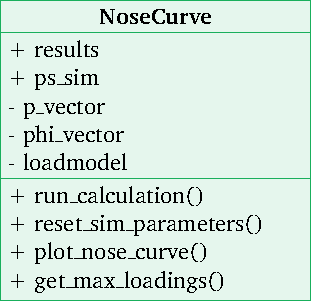
\includegraphics[width=.9\linewidth]{tikz_graphics/images/class_diagram_nosecurve_red.pdf}
        \caption{Class diagram of the NoseCurve class in the package diffpssi}
        \label{fig:nose-curve-characterization}
\end{wrapfigure}
The implementation of the nose curve generation is realized as a class in the package {\itshape diffpssi.stability$\_$lib.voltage}.
Its class diagram with all attributes and methods is shown in \autoref{fig:nose-curve-characterization}, an extended version is included in \autoref{app:nose-curve}.
For an easy and generic use of the {\itshape diffpssi} package, {\itshape PowerSystemSimulation} objects are used, as well as the function {\itshape do$\_$load$\_$flow()} from the package.

As the afore mentioned idea, the method for running the calculation is a iterative wrapper of the load flow calculation. 
This can be as well applied for mutiple busses as a list input.
At first, the grid and therefore models of the {\itshape PowerSystemSimulation} object has to be cleared with the method {\itshape reset$\_$sim$\_$parameters()}.
Then the active power vector is iterated as load input, together with the power angle $\phi$ for the reactive power in the model.
Important to note here, is the usage of an {\itshape **kwargs} argument.
The callable for the model is called with load parameters for each load bus as the Bus name, and a list with active and reactive power.
The initials of this grid callable are used as the standard values, so only one bus can be varied at a time.
The result is saved as a {\itshape pandas DataFrame} in a dict, with the keys being the bus names.

The method {\itshape plot$\_$nose$\_$curve()} is used to plot the results, and is using the {\itshape matplotlib} package.
Further, the method {\itshape get$\_$max$\_$loadings()} can provide details about the critical point.
Giving back a dict with keys as bus names, the values itself are dicts with key of the power angle parameter $\tan \phi$ and the values as {\itshape pandas DataFrame}.
The contained details are maximum active power $P_\mathrm{max}$, the reactive power $Q$ at this point, and the voltage magnitude $\vert \underline{V} \vert$ at the bus.

\sidenote{Parameter variation Nose Curves}
Additionally, the method set \textit{run$\_$variation$\_$calculation()} and its connected automated plotting method \textit{plot$\_$nose$\_$curve$\_$variation()} aims to calculate a nose curve parameter set uder variation of a system parameter variation.
This is realized through a callable function, enabling access to the desired object attribute.
Additionally a list of variation values as to be handed over, for iteration over it and saving the result to a dictionary.
This dictionary then can be plotted or accessed over the object as attribute.
The \acs{OLTC} tap dependent Nose Curves from \autoref{fig:oltc-nose-curve} are generated by this functionality

\subsubsection{Results of the Nose Curve Generation}

The following figure \autoref{fig:nose-curve-simple-grid} shows the generated nose curve for a simple grid as illustrated in \autoref{fig:single-line-voltage-stability}.
The grid is characterized at Bus 1, with a varying power angle as parameter $\tan \phi$.
The power angle $\tan \phi$ is used to vary the power factor of the load, thus representing different load characteristics, as
\begin{align}
        \tan \phi &= \frac{Q}{P}. \notag %\label{eq:tan-phi} \\[6pt]
\end{align}
Displayed are a few combinations with different load characteristics, leading to a different possible maximum acitve power transfer.
\autoref{fig:nose-curve-simple-comp} shows the comparison between the analytical calculation and the implemented solution.
The analytical calculation is carryied out with the method described in \autoref{sec:analytical-voltage-stability}.
For this specific example, the complete calculation, including the set of used parameters, is shown in \autoref{app:analytical-nose-curve}.
What seems conspicious is the missing lower part of the curve, meaning the second possible solution when solving the power flow equations.
Although this seems like a major drawback, the resulting curve contains all the necessary parts, where a stable solution can occur. \quelle
The solution is reaching exactly until the critical point of power transfer.

\begin{figure}[htbp!]
        \centering
        \includegraphics[width=\linewidth]{development_files/theoretical/plots/simple_load_B1_nose_curve.pdf}
        \caption[Examplary generated nose curve for a simple generator - load grid]{Examplary generated nose curve for a simple generator - load grid for various power angle level parameters $\tan \phi$; Applied on the grid of \autoref{fig:single-line-voltage-stability} with a characterization at Bus 1}
        \label{fig:nose-curve-simple-grid}
\end{figure}

\begin{figure}[htbp!]
        \centering
        \includegraphics[width=\linewidth]{development_files/theoretical/plots/simple_load_B1_nose_curve_w-theoretical.pdf}
        \caption[Comparison between the analytical calculation and the implemented solution]{Comparison between the analytical calculation and the implemented solution}
        \label{fig:nose-curve-simple-comp}
\end{figure}


%%%%%%%%%%%%%%%%%%%%%%%%%%%%%%%
\subsection{Combination of Static Methods with Time Domain Solutions}
\label{sec:comb-time-dimension}

Adding a \acs{TDS} to the static Nose Curve plot is fairly simple and straight forward.
The basic idea is gathering the demanded power by the load as additional recorder function, to overlap the diomensions voltage and power in the static plot.
Adiitionally using color alteration for the time dimension is keeping the evolvement information as well.
This data is then just added to the plot of Nose Curves.
The backgorund on why this could give a valuable inside, is simply looking into how close to the static solutions of the grid can the system stay under dymanic equalization and control processes.
The static solutions should theoretically the long-term solutions or states after the equalization processes.
As this dynamic solution is also conditional to the machine and machine controls for example, it could give explanations about missing capabilities from this point, as the nose curves just express the network limits.

Necessary for gathering the missing power information, the method \textit{get$\_$value()} has to be added to the static model \textit{Bus} as well.
There, specifically the apparent power $S$ is calculated through the sum of the models current injections.
With the basic relations
\begin{align}
        S&=\underline{V} \cdot \underline{I}^* \notag, \\
        P&=\mathfrak{Re} \{S\}\text{, and} \notag \\
        Q&=\mathfrak{Im} \{S\} \notag
\end{align}
one can then acces the active power as recorder attribute. 
Important to note here is, that the curret injection of a simple load cannot be calculated by default, as this model is solely adding a contribution to the admittance matrix of the system.
Therefore this model does not consider curretn injections.
As proposed work around, a load attribute \textit{i$\_$inj} is calculated in each iteration of the method \textit{get$\_$admittance()} in the static model \textit{Load} with the relation
\begin{align}
        \underline{I}_\mathrm{inj}=S_\mathrm{load}(t) \cdot \frac{S_\mathrm{n,sys}}{\underline{V}(t)^*}. \notag
\end{align}

% \commenting{
%         Idea here: Show the dynamic RMS simulation results in the quasi-staionary assessment techniques.
%         These are static solutions to the network, the electromechanic equalization processes should on a long-term watch result in these states.
%         With controls of the machines etc. one can obtain more or less a following of the static solutions until a certain point.
%         If the grid, or the machine, or its control units are stronger, a certain (heavy) level of load increase can be better and faster compensated.

%         Maybe interesting: Can the faster FSM not only increase the time until Voltage envelope is violated, but extend the transferred power as well?        
% }
        
%%%%%%%%%%%%%%%%%%%%%%%%%%%%%%%
\subsection{Using Voltage Envelopes for Criticality Evaluation}
\label{sec:comb-rating-tool}

\sidenote{Class\\ViolationIntegral}
The afore described method from \autoref{sec:stability-indices}, the \acs{TVI} is implemented as seperate class \textit{ViolationIntegral} in the package \textit{diffpssi}.
Automated simulations are not considered, as they do not add significant practicability.
Therefore, simply the results vector is just handed over.
The class diagram is displayed in \autoref{fig:class-violation-integral}.

\begin{figure}[htbp!]
        \centering
        \missingfigure{Class diagram VioolationIntegral}
        \caption[Class diagram for the class ViolationIntegral]{Class diagram for the class ViolationIntegral}
        \label{fig:class-violation-integral}
\end{figure}

As afore described, not only the mathematical describable envelopes are added, but the Machine Type II \acs{FRT} curves when connecting to the medium voltage grids from \autocite{vde-tar_2018,vde-tar_2023} are added as well.
Both envelopes are implemented as a function dependent on the time, giving back a vector in the length of the time vector and being comparable to the bus voltage solution from the power system simulation object.
Envelope parameters can be set with the function \textit{set$\_$env$\_$paramms()}, but can as well be read out through the function \textit{get$\_$env()}.
Here the same logic applies as with the envelope functions before, as a vector with the length of the time vector is given back.

\begin{figure}[htbp!]
        \centering
        \missingfigure{Class diagram CriticalTimes}
        \caption[Class diagram for the class CriticalTimes]{Class diagram for the class CriticalTimes}
        \label{fig:class-critical-times}
\end{figure}

\sidenote{Class CriticalTimes}
The class \textit{CriticalTimes} is added as well as displayed in \autoref{fig:class-critical-times}.
It is used to enable a calculation of all time steps, where the envelope(s) are violated.
The method accounts just the time stamp, where the envelope is cut from inside to outside, instead of returning all time steps outside of the envelope(s).
The envelopes can be added and results can be calculated through handing over a bus voltage result with time vector.
Results are stored as an attribute as well.
The enevelope functions are re-used from the class \textit{ViolationIntegral}

%%%%%%%%%%%%%%%%%%%%%%%%%%%%%%%
%%%%%%%%%%%%%%%%%%%%%%%%%%%%%%%
\section{Summary in Short and Simple Terms}

\commenting{
        Transformer equipment:
        \begin{itemize}[nosep]
                \item Two models -> One has to look out for which and which circumstances and definitions
                \item Phase shifting not possible -> Would be complex number instead of rational 
                \item Standardized interfaces and design
        \end{itemize}
        Voltage Rating Tool:
        \begin{itemize}[nosep]
                \item Combination of static and dynamic indices -> Evaluation of network capabilities, machine relation to that, evaluation of dynamic behavior, and assessment of the events
                \item (Static) Indexes would classify the distance / reserves of the system
                \item One number to compare for more or less stable
                \item Finding the weakest busses poossible with that -> Regarding complexer networks
        \end{itemize}
}
%!TEX root = ../main.tex

% \part{Enhancing the System Stability Assessment}

%%%%%%%%%%%%%%%%%%%%%%%%%%%%%%%
%%%%%%%%%%%%%%%%%%%%%%%%%%%%%%%
\chapter{Verification Setup and Results}
\label{chap:verification}

\begin{textblock*}{.7\textwidth}(70mm-\offset,25mm-\offset)
    \begin{fquote}[Mark Twain]
        If you tell the truth, you don't have to remember anything.
    \end{fquote}
\end{textblock*}

%%%%%%%%%%%%%%%%%%%%%%%%%%%%%%%
\section{Representative Electrical Networks}
\label{sec:networks}

The following section shall introduce the used power systems in the simulation with the Python framework, considering verification, and also extension meaning the performed case studies in \autoref{chap:case-study}. 
The models are chosen to represent different network sizes and complexities, thus allowing the objective of graded interaction levels of the developed (transformer) model. 
The models are based on the work of \textcite{machowski_2020}, \textcite{kundur_2022}, \textcite{IEEELoadModeling_2022}, and \textcite{vancutsem_2020}.

\subsubsection{Single Machine Infinite Bus (SMIB) Model}

One very popular and thus powerful electrical network for the verification of power system stability is the \acs{SMIB} model. 
It is a compact and simplified model of a power system, allowing easy analytical calculation, verification and development. 
Mutual influences are comparably simple to understand and calculate, as the infinite bus bus is acting as a fixed grid connection point with a large adjoining grid. 
The generator is connected to the bus bar via a transmission line and a transformer. 
The model was largely discussed by \textcite{kundur_2022}, and is shown in Figure \ref{fig:smib-model}. 
The generator and the \acs{IBB} are represented by synchronous machines, developed and discussed by \textcite{kordowich_2023}. 
The specific model details are included in \autoref{app:smib-model}, additionally the simulation setup for verification is described in \autoref{tab:smib-model}.

\begin{figure}[htb]
    \centering
    \vspace{12pt}
    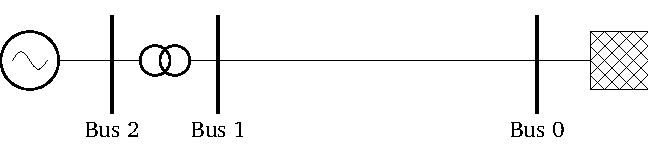
\includegraphics{tikz_graphics/images/smib_model.pdf}
    \vspace{12pt}
    \caption[]{\acf{SMIB} model for verification and validation of the Python framework; own figure after \autocite{machowski_2020,kundur_2022}}
    \label{fig:smib-model}
\end{figure}

\begin{table}[htb]
    \caption[Simulation Setup for validation of the $\Pi$-modeled transformer]{Simulation Setup for validation of the $\Pi$-modeled transformer; considering a transforming ratio $\underline{\vartheta} \neq 1$ and $\underline{\vartheta} \in \mathbb{C}$}
    \label{tab:smib-model}
    \vspace*{12pt}
    \centering
    \small
    \begin{tabularx}{\textwidth}{Xr}
        % \toprule
        \textbf{Parameter} & \textbf{Value} \\ \hline
        \toprule
        Generator inertia $H$ & 3.5 s \\
        Generator damping $D$ & 0.1 p.u. \\
        Generator resistance $R$ & 0.01 p.u. \\
        Generator reactance $X$ & 0.1 p.u. \\
        Transformer resistance $R$ & 0.01 p.u. \\
        Transformer reactance $X$ & 0.1 p.u. \\
        Transmission line resistance $R$ & 0.01 p.u. \\
        Transmission line reactance $X$ & 0.1 p.u. \\
        \bottomrule
    \end{tabularx}
\end{table}

Further, this model shall be slightly modified according to \autoref{fig:smib-model-mod}. 
A load is added at the secondary bus of the transformer, the rest of the system is kept. \autoref{tab:smib-model} already contains this modification.

\begin{figure}[htb!]
    \centering
    \vspace{12pt}
    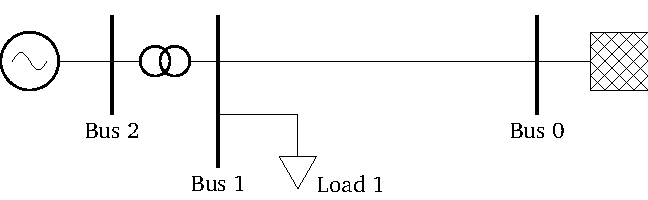
\includegraphics{tikz_graphics/images/smib_model_with_load.pdf}
    \vspace{12pt}
    \caption[]{Modified \acf{SMIB} model with additional load}
    \label{fig:smib-model-mod}
\end{figure}

\subsubsection{Simple Single Machine Load Model}

Following model is often recommended \quelle for easy voltage control studies, in explicit for \acsp{OLTC}. 
Similar to the \acs{SMIB} model, it consists from one synchronous generator, busses, and lines in a single branch. 
The \acs{IBB} is thus removed and changed to a load. 
This two element type o configuration allows for an easy analytical calculation of voltage stability and control. 
Although this thesis is focussing on \acs{OLTC} transformers, the model is extended with one in between. 
A single line representation is depicted in \autoref{fig:single-line-voltage-stability}.

\begin{figure}[htb!]
    \centering
    \vspace{12pt}
    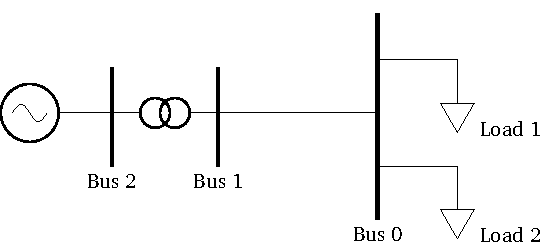
\includegraphics{tikz_graphics/images/sm_load_model.pdf}
    \vspace{12pt}
    \caption[Single line representation of a simple single machine load model]{Single line representation of a simple single machine load model; own illustration with characterstics from \quelle}
    \label{fig:single-line-voltage-stability}
\end{figure}

Further details about its configuration and simulation setup are included in \autoref{app:single-line-model}. 
It should be noted, that simple load models are not useful for simulation of this example network. 
Usually constant Z models are used as loads, therefore simulation results can be misleading and not showing desired effects or voltage instability mechanisms \quelle. 
% \commenting{The simulation framework is extended with XX types of load models, to satisfy the requirements of the single machine load model, and a connected stability assessment.}

% \subsubsection{IEEE Nine-Bus System}

% \subsubsection{Nordic Test System}

%%%%%%%%%%%%%%%%%%%%%%%%%%%%%%%
%%%%%%%%%%%%%%%%%%%%%%%%%%%%%%%
\section{Validation Steps}

Following section shall guide through the validation process.
Beginning with the new transformer $\Pi$-model, therefore lokking deeper into characteritic behavior dependent on the rated apparent power and the longitudinal ratio.
Proceeding with the three modeled control circuit and their behavior.
Lastly, some applied plausibilisations shall be done with the implemented voltage stability rating tools.

%%%%%%%%%%%%%%%%%%%%%%%%%%%%%%%
\subsection{Validation of the Modeled Transformer with Variable Tap Position}

As mentioned before, the base validation is concerning the basic transformer model.
For this, a parameter variation and comparison to the results from \textit{DIgSILENT PowerFactory} shall give a good representation of the accuracy.
The varied parameters are the apparent rated power $S_\mathrm{n}$ of the transformer, the longitudinal ratio $\vartheta$, the transformer reactance $X$, and the phase shifting angle $\phi$, resulting from the applied vector group.
The last two parameters are not included, because the transformer reactance is passively included in the ratio.
The reason for excluding the vector angle $\phi$ relies in the not congruent results.

\subsubsection{Variation of the Apparent Power}

\begin{figure}[htbp!]
    \centering
    \includegraphics[width=\linewidth]{development_files/validation/data/s_n_comp_errors.pdf}
    \caption[Model error comparison concerning the variation of the rated apparent power]{Absolute errors while comparing the tool \textit{diffpssi} with the software \textit{DIgSILENT PowerFactory}; One plot each for every parameter variation, concerning the errors for each bus}
    \label{fig:valid-s-errors}
\end{figure}

The rated apparent power $S_\mathrm{n}$ shall be varied in three steps acoording as described in \autoref{eq:variation-s-n}. 
The used grid model is the afore described \acs{SMIB} model. 
This is showing some predictable dynamics, but enabling a relative uncomplicated and easy to overview troubleshooting, if necessary.
The used grid parameters staying as described before, only the transformer apparent power is varied.
\begin{align}
    S_\mathrm{n} \in \{ 1100; 2200; 4400 \}~\mathrm{MVA} \label{eq:variation-s-n}
\end{align}
The used model for the comparative tool \textit{DIgSILENT PowerFactory} is as well included in the \textit{diffpssi} repository.
A plot of both results is depicted in \autoref{fig:valid-s-compl}
Looking deeper into one parameter, but plotting both tools in one diagram, \autoref{fig:valid-s-1100} in \autoref{app:add-validation-plots} is showing the results.
The three split diagrams account for each bus, where nearly no difference is obtainable.

Supporting this observation is the comparison of errors as illustrated in \autoref{fig:valid-s-errors}.
The error is not exceeding $0.005$ p.u. in any case.
One note to make here is, that due to the per unit nature of the calculation the initial values are often around $1$ p.u.
Therefore the seperate calculation of a relative error is neglected, as the absolute error is containing more information, and thus not surpassing the feel of relative nature.
Following this argumentation, the maximum relative error shall be around $0.05$ \% for this parameter variation.

\subsubsection{Variation of the Longitudinal Ratio}

\begin{figure}[htbp!]
    \centering
    \includegraphics[width=\linewidth]{development_files/validation/data/theta_comp_errors.pdf}
    \caption{Comparison of different varied parameters between \textit{diffpssi} and \textit{DIgSILENT PowerFactory}}
    \label{fig:valid-ratio-errors}
\end{figure}

In similar way as the validation approach for the rated apparent power, the longitudinal ratio shall be varied. 
Therefore the same network, with identical parameters is used, only that at this time the rated apparet power is fixed as well and the longitudinal ratio of the transformer is fixed during the simuatlion time according to following variation:
\begin{align}
    \vartheta \in \{ 0.9; 1.0; 1.1 \}~\mathrm{p.u} \label{eq:variation-ratio}
\end{align}
Looking into the results, in the same form as previously.
On the left side of \autoref{fig:valid-ratio-comp} is the result from the Python module \textit{diffpssi}, the right side is accounting for the validation tool \textit{DIgSILENT PowerFactory}.
The focussed comparison for the fixed ratio of $0.9$ p.u. is included in \autoref{app:add-validation-plots}.
As well \autoref{fig:valid-ratio-errors} is showing absoulte errors in the same manner.
The obtainable error for this case is comparably high, excluding for the reductive ratio of $0.9$ p.u.
This increasing with simulation time, to around a factor of 10 of the other errors. 
But still, this error is in a margin of lower than $1$ \%. 


%%%%%%%%%%%%%%%%%%%%%%%%%%%%%%%
\subsection{Parenthesis: Accountability of the Load Model}
\label{sec:validation-load-model}

\begin{figure}[htbp!]
    \centering
    \includegraphics[width=\linewidth]{development_files/validation/data/comparison_z_load.pdf}
    \caption[Comparison of the constant impedance model for each bus]{Comparison of the constant impedance model for each bus between the Python module \textit{diffpssi} and \textit{DIgSILENT PowerFactory}}
    \label{fig:z-comp}
\end{figure}

A static load model with quadratic dependency on the voltage had been implemented in the Python module before.
The load model can thus be classified as constant impedance model, or often referred as constant $\underline{Z}$ model \autocite{IEEELoadModeling_2022}. 
As this is playing a role in the chain of accumulating errors, following parenthesis shall give a feeling what contibution is generated through this load model.
For this evaluation the Single Line with Load model from \autoref{sec:networks} is used, with a load jump from $P=400\text{ MW}$ to $P=800\text{ MW}$ at the time stamp $1$ s.
The overall simulation time is set to $20$ s.
Other parameters are set as described in \autoref{sec:networks}.

\begin{figure}[htbp!]
    \centering
    \includegraphics[width=\linewidth]{development_files/validation/data/z_load_error.pdf}
    \caption[Absolute error comparison of the constant impedance model]{Absolute error of the already implemented constant impedance model over time; Accounted for both busses zero and one}
    \label{fig:z-load-error}
\end{figure}

\autoref{fig:z-comp} is showing the time series computation for each bus compared between both tools \textit{diffpssi} and \textit{DIgSILENT PowerFactory}.
Visible is the more extreme pronounciation of the overshoot and the convergence value over time of the Python package.
Looking at the absolute error comparison for each bus in \autoref{fig:z-load-error} showing a increase over time, and peak offsets of around $0.006$ p.u.
This accounts for an error lower than $1$ \% in this scenario.

%%%%%%%%%%%%%%%%%%%%%%%%%%%%%%%
\subsection{Validation of the OLTC Control Schemes}
\label{sec:validation-oltc-schemes}

To begin with this section of control scheme validation, the basic strategy accounted for all the considered models and verification setups.
The characterizations of the control loop feedbacks has already been carried out in the modeling chapter \autoref{sec:modeling-tap-changer-control}.
To validate the in-simulation behavior of the control loops, two different scenarios are accounted for the \acs{OLTC} and the \acs{FSM}.
First, the Simple Load against Machine grid is used with the declared parameters as in \autoref{sec:networks}.
To bring the system in a dynamic state, a load increase is added at the simulation time point $1$ s.
All differing values are pointed out in the validation result presentation later on.
Secondly, the more complex version of a \acs{SMIB} model with a connected load at the middle bus is used to account for a different scenario including a load flow direction change.
It would be expected, that neither \textit{DIgSILENT PowerFactory} or \textit{diffpssi} would be able to react on this supposed load flow direction change.

\subsubsection{Standard Discrete OLTC Control}

The first consideration for validation of the \acs{OLTC} control is the simple load model against a machine.
The applied load change is shifting the real power of the load from $P=400\text{ MW}$ to $P=800\text{ MW}$ at the simulation time $1$ s.

\begin{figure}[htbp!]
    \centering
    \includegraphics[width=\linewidth]{development_files/validation/data/comp_oltc_simple-load.pdf}
    \caption[Time Domain Result of the OLTC control scheme applied on the extended \acs{SMIB} network]{\acf{TDS} of the standard discrete \acs{OLTC} control scheme; Result of the extended or modified \acs{SMIB} model with additional load}
    \label{fig:comp-oltc-simple}
\end{figure}

When comparing the time series solution from \autoref{fig:comp-oltc-simple} for both bus voltages, one can obtain a similar course of the curves. 
Only a small deviation is visible, the tap changes of the \acs{OLTC} clearly visible and around the same times.
A similar picture is drawn, when loooking at the absolute error of this scenario in \autoref{fig:comp-oltc-error-simple}.
In the areas of time, where the switching occurs, peaks of errors are visible, showing just the less congruent development of bus voltages and switching.
After the half of the simulation time, a new (quasi-) stationary state is showign a static offset or error.
This error is around $0.005$ p.u., showing a slightly higher error than when looking at this scenario without the tap changing transformer in \autoref{sec:validation-load-model}.

\begin{figure}[htbp!]
    \centering
    \includegraphics[width=\linewidth]{development_files/validation/data/error_oltc_simple-load.pdf}
    \caption[Bus and Error Comparison for the standard discrete \acs{OLTC} scheme applied on the extended \acs{SMIB} model with load]{Comparison of the standard discrete \acs{OLTC} control scheme applied on the extended \acs{SMIB} model with additional load; One plot for each bus with data from \textit{diffpssi} and \textit{DIgSILENT PowerFactory}; Additional plot for showing the absolute error for each bus}
    \label{fig:comp-oltc-error-simple}
\end{figure}

Some blibla

\begin{figure}[htbp!]
    \centering
    \includegraphics[width=\linewidth]{development_files/validation/data/comp_oltc_ext-smib.pdf}
    \caption[Bus and Error Comparison for the standard discrete \acs{OLTC} scheme applied on the extended \acs{SMIB} model with load]{Comparison of the standard discrete \acs{OLTC} control scheme applied on the extended \acs{SMIB} model with additional load; One plot for each bus with data from \textit{diffpssi} and \textit{DIgSILENT PowerFactory}; Additional plot for showing the absolute error for each bus}
    \label{fig:comp-oltc-control-ex-smib}
\end{figure}

\begin{figure}[htbp!]
    \centering
    \includegraphics[width=\linewidth]{development_files/validation/data/oltc_ex-smib_signals.pdf}
    \caption[Internal signals of the \acs{OLTC} control in the extended \acs{SMIB} model]{Internal signals of the \acs{OLTC} control in the extended \acs{SMIB} model; a) the longitudinal transformer ratio $u_\mathrm{l}$ or mathematically referred as $\vartheta$, b) the deadband filtered voltage difference signal $v_\mathrm{dead}$}
    \label{fig:int-signals-ext-smib-oltc}
\end{figure}

\subsubsection{Fast Switching OLTC Control}

As described in the modeling chapter, specically \autoref{sec:modeling-tap-changer-control}, of the \acs{FSM} module control, two control methods are implemented.
First, as described in the paper of \textcite{burlakin_2024} with preferring the switching of the \acs{FSM}, and secondly the dependence on the function of tap skipping.
As only the last model is available in the comparative tool \textit{DIgSILENT PowerFactory}, only this can be compared and validated. 
The other control scheme is implemented similarly and used as well for futher studies.

\commenting{
    Due to some factors (which?), the control becomes more off the more states it has -> FSM seems not good, OLTC okay, Loads nearly identical.
    This means there must be differences within the static / dynamic time steps, the load model parameterization, The load model behavior, the model of the transformer itself, the discrecity of the transformer tap control etc.

    This means: Showing, that the control algorithmics is switching correctly, no matter what the result does look like at the bus voltages e.g.
}

%%%%%%%%%%%%%%%%%%%%%%%%%%%%%%%
\subsection{Voltage Stability Rating Plausibility}

\commenting{
    Place results here, looking at: off nominal tap ratio, and with off nominal phase shifting (e.g. $110^\circ$)

    Things to illustrate:
    \begin{enumerate}
        \item Validity of Top Branch Nose Curves: Analytical and PowerFactory; Simple Network and e.g. IEEE 9-bus 
        \item Analytical Validity OLTC ratio dependent Nose Curves
        \item Time Domain Projection: Dependence and Stability in transient scenarios vs. continous load increase; Dependence on Machine Controls; Dependence on Apparent Power Capacity of machine 
    \end{enumerate}
}

%%%%%%%%%%%%%%%%%%%%%%%%%%%%%%%
\section{Model Limitations and Improvements}

\section{Summary in Short and Simple Terms}
%!TEX root = ../main.tex

% \begingroup
% \newgeometry{left=2.5cm,right=2.5cm,top=2.5cm,bottom=2.5cm}
% \part{Practical Application: Simulation}

% \endgroup

%%%%%%%%%%%%%%%%%%%%%%%%%%%%%%%
%%%%%%%%%%%%%%%%%%%%%%%%%%%%%%%
\chapter{Case study}
\label{chap:case-study}

\begin{textblock*}{.7\textwidth}(70mm-\offset,25mm-\offset)
    \begin{fquote}[Narcotics Anonymous]
        Insanity is doing the same thing, over and over again, but expecting different results.
    \end{fquote}
\end{textblock*}

\commenting{
    In the interest of investigation / the Case Study are:
    \begin{itemize}[nosep]
        \item Influence of switching times on stability margin/begin of destabilization,
        \item Influence of max. ratio change per switching event, and
        \item Influence on different test systems (destabilization mechanisms).
    \end{itemize}
}

\section{Scenario setting}

\commenting{
    Does it make sense to structure like that? (Scenarios - Simulation - Results)

    Or is it a better idea thinking in terms of specific \glqq use cases\grqq~as sections:
    \begin{itemize}[nosep]
        \item What happens under strong grid conditions? -> Section: Strong grid condition behavior
        \item What happens under weak grid conditions? -> Section: Weak grid condition behavior
        \item Strongly interconnected grids
        \item Widely extended linear string grids
        \item Section: Use case of Wind farm integration
        \item Influence on transient stability: SMIB model with and without OLTC
    \end{itemize}
}

\subsubsection{Influence of FSM on Machines and their stability criterions}

\commenting{Thinking of Rotor Angle Stability, maybe considered by an EAC implementation?
What does the fast Switching, esp. at up to 8\% of the nominal voltage, do to the machines?}

\subsubsection{Novel Control Strategy FSM}

\commenting{Thinking of fast and slow voltage gradients: fast gradients are compensated by the FSM, slow gradients are compensated by the OLTC. Therefore optimal utilisation of injected damping moment of the FSM. 

Also thinking of different presets of the OLTC and FSM, which are tried to keep constant. Different grid operators can utilize for typical grid conditions of over- or undervoltage at \acs{PCC}.

Following contains:
\begin{itemize}
    \item Implemetation of different logic
    \item Testing of presets and switchin logic
    \item Damping moment beneficial?
\end{itemize}
}

\subsubsection{Possible Extension for Power Flow congruent Control}

\commenting{Extension in the Control Algorithm to decide which Bus has to be regulated, to avoid contrairy actions of the OLTC and FSM against the power flow. Therefore not decrease of stability, but increase. Possible Application: Grid coupling Transformers, Battery Storage assisted Virtual powerplants, etc.

For this thinking maybe another control strategy is relevant:
\begin{itemize}[nosep]
    \item No setpoint from a load flow day-ahead or similar time frame; but rather current load and bus voltages are considered
    \item Not the deviation of one transformer bus voltage from a setpoint, but the deviation between the two bus voltages is relevant
    \item Maybe the absolut deviation to the optimal bus voltages at the current load situation is relevant  
\end{itemize}

Big general problem: In which direction does the OLTC / the FSM have to swith? In some cases, the direction is not correct, in some it is correct.}

\section{Simulation}

\section{Results}
%!TEX root = ../main.tex

% \addtocontents{toc}{\protect\addvspace{2.25em}}
% \bookmarksetup{startatroot}

%%%%%%%%%%%%%%%%%%%%%%%%%%%%%%%
%%%%%%%%%%%%%%%%%%%%%%%%%%%%%%%
\chapter{Discussion of the Results}
\label{chap:discussion}

\begin{textblock*}{.7\textwidth}(70mm-\offset,25mm-\offset)
    \begin{fquote}[Joseph Joubert]
        The aim of argument, or discussion, should not be victory, but progress.
    \end{fquote}
\end{textblock*}

This chapter discusses all chapters combined, with found aspects, expected or unexpected behaviors, or comparisons.
Singular discussions in each chapter are avoided, to maintain a high level view on the \acs{FSM}.
Nevertheless, details do matter here and are included in the summarized evaluation.
The structure of this chapter does not hold up with the before used structure.
This shall make use of the combined discussion, more orientating on the found aspects, than the done work. 

%%%%%%%%%%%%%%%%%%%%%%%%%%%%%%%
\section{Integration in diffpssi}

First, the done implemetation in the tool of choice, \textit{diffpssi} is discussed.
Conspicuities, current existing restrictions of the assessments, as well as missing ones are elaborated.
At last, a further idea of utilizing the benefits of \textit{diffpssi} is illustrated.

\subsubsection{Implementation of the Models}

\sidenote{Transformer equipment}
As the results for the model validation are already described in \autoref{chap:verification}, there is a relatively short discussion on the accounted errors.
The errors show overall low values in comparison to the commercial software \textit{DIgSILENT PowerFactory}.
The variable ratio transformer itself has errors of maximum in the one digit percent range.
As this can also account for solver or time step issues, the Python framework is giving competitive results.
Considering the injected errors of the already implemented load model, the results of the control schemes are even less error prone.
It is assumed, that because of the longer time period of holding the voltages closer to the reference value, the error can even be dropped. 
Peaks only occur during the switching of tap positions of the \acs{OLTC} or \acs{FSM}, where not only solver issues, but the time filtering or else can accumulate for a very short time.
The logic of the \acs{FSM} controls only shows correct results, as also confirmed by \autoref{chap:case-study}.

\sidenote{Voltage stability tools}
As the only comparison for the voltage stability tools can be drawn with respect to the Nose Curves, these deliver very good results as well.
The curves are congruent, making it hard to visually spread them apart, both compared analytically and with \textit{DIgSILENT PowerFactory}.
The other tools show a logic beahavior, as the visual inspections allow for the same claims as the algorithmics.
Only one results seems somehow suspect, as the \acs{TVI} calculation shows even a violation area for the stable cases of one bus in \autoref{chap:case-study}, specifically \autoref{tab:case1-tvi}.
It was not possible to investigate on the cause of this unexpected behavior so far.

\subsubsection{Currently Existing Restrictions}

\sidenote{General}
However there are some restrictions to the Python framework, considering the applicability on voltage stability studies.
As only static load models or synchronous machines can be represented as loads, the characteristics of a realistic grid is very limited.
Further, \textit{diffpssi} only contains the constant impedance load model.
Often pointed out by \textcite{cutsem_1998}, \textcite{kundur_2022}, or \textcite{danish_2015}, the bottleneck for remaining stable voltage levels are induction machines.
These are currently not available in \textit{diffpssi}, so a lot of studies will not show the same characteristics as one would be able to conduct with comparative (commercial) software.
If this model would be available in the future, even combinations with inverters as supporting reactive power source, or connected controllers could be tested very easily.
Nevertheless this package is suited well for basic developments of single components, such as a tap changer controller.
The logic and algorithmics are implemented fast and allow for a transparent debugging.
The easy and close connection with Python does make the package especially great for direct evaluation of results.
Either in plotting and visualization, for statistic assessments, or even batch calculations, but as well for futher processing and calculations with the results. 

\sidenote{Transformer related}
Additionally, the variety of available transformer types is also very limited.
There are a lot of different technologies possible to consider, from line drop compensations over phase shifting transformers or \ac{WAMPAC} approaches.
Even simpler things, like parallel transformers, and the related complications with circular currents cannot be adressed with \textit{diffpssi} or this thesis.
Regarding transformers, \textcite{sarimuthu_2016} is presenting a review paper considering a few of these topics as an overview.
When looking at the possible damping factor from the \acs{FSM} control, one could also think of something like a \glqq machine drop compensation\grqq~for futher development.

\subsubsection{Missing Assessments in this Thesis}

Looking at the integrity of the implemented models, there are a few edge cases or considerations, which are excluded.
These however could be beneficial, depending on the application of the technologies.
A parameter variation for the \acs{FSM} characteristics has not been carried out.
The standard values presented by \textcite{burlakin_2024} have continuously been used, as they are comparable and show conclusive results so far.
However for different use cases, voltage and power levels or dynamic loads, also other parameters have to be considered.
On top of that and regarding the different basic use cases for transformers, only a transformer connecting a machine was used in this thesis.
As transformers for complete power plants, virtual power plants, connecting \acp{BESS}, grid coupling, etc. \autocite{schwab_2022} is usually also covered, these application could also be of interest.
The later on discussed control improvements could be not implemented and evaluated as well.

\subsubsection{Increasing the Benefits of diffpssi}

One further interesting application of the Python package \textit{diffpssi} is the possibility for parameter differentiation based on \textit{PyTorch}.
\textcite{kordowich_2023} uses this for an optimization approach, allowing to optimize certain defined simulation parameters to acquire a defined system behavior.
For example, the dampening of the synchronous machine swinging after a short-circuit event can be increased.
The idea is, to apply this method also on the \acs{FSM} control scheme, thus optimizing its behavior, e.g. number of switch operations, power oscillation damping or other things.
As the tap changer model and its control is already implemented, one could make use of this functionality.

%%%%%%%%%%%%%%%%%%%%%%%%%%%%%%%
\section{Evaluation Current FSM Control}

% After the toolchain, the content of interest is more central.
The \acs{FSM} control schemes are analyzed in the following, which characteristics, benefits, and current drawbacks exist.
Lastly, further investigations on the control schemes are named, as they are not included in this thesis any more.

\subsubsection{Characteristics of the FSM controls}

The results as differences are mainly illustrated in the \autoref{chap:case-study}, but in some terms visible in \autoref{chap:verification} as well.
The increased stabilization through the \acs{FSM} control can be confirmed for both switching only with the \acs{FSM} part and with both dependent on the voltage deviation.
% The increased stabilization through the \acs{FSM} control can be confirmed, for both only switching with the \acs{FSM} part, but as well with both dependent on the voltage deviation.
The envelopes are not cut after the fault at all, while the \acs{OLTC} scheme can only postbone the rapid fall a few seconds.
Even if one would want to argue, that with the accounted \acs{FSM} schemes, the control has a wider range of operation.
One can clearly see in the \acs{TDS}, that the rapid intervention of the \acs{FSM} is holding the voltage closer to the reference value a lot earlier.
On top of that, considering the \acs{FSM} preferring control, no single switch of the \acs{OLTC} has occured, and yet the system is stable for a longer period of time.

One main finding in this thesis is the back propagation of the \acs{FSM} control on the oscillation behavior of synchronous machines after the fault.
Clearly, an influence through the ratio is visible, if not even the crucial part to stabilizing the whole system after the fault.
Thus the \acs{FSM} as well help stabilize a system with more and faster dynamics compared to the \acs{OLTC}.
Another finding is the accounted deaf band in \autoref{sec:validation-fsm-schemes}, which has especially be considered for different combinations of deadband size and switching magnitude of the \acs{FSM}.
As one can also see in \autoref{fig:case1-trans-ratio}, the \acs{FSM} ratios are not vastly different from the \acs{OLTC}, but just are coarser per tap change.
As this is leading to a lot less switches of the \acs{OLTC} and therefore less use of the mechanical switching contacts, both \acs{FSM} controls seem to have an optimal behavior somewhere in between them.
Utilizing the \acs{FSM} where possible and only short- or mid-term fluctuations occur.
And using the \acs{OLTC} where the load flow and voltage has to be influenced long-term, enabling the most dyanmic capabilities.   

\subsubsection{Further Investigations}

Regarding the further investigations of the \acs{FSM} control schemes, one aspect has to mentioned.
The next step would be an assessment with machine controllers, as gaining insights on how these controllers would interact.
If one would want to use a \acs{FSM} equipped controller as a machine or power plant connector to the grid, this is a crucial part.
As the short control times already have an influence on the machine dynamics, they could also interfer with the short term considering machine controllers, like exciters \autocite{machowski_2020}.
This expectation holds true for inverter controllers as well.

Regarding the topic increasing voltage stability through a \acs{FSM}, an even bigger potential is the application on to a phase shifting transformer in particular.
As these transformers are also able to change the voltage angle difference between two nodes, this could have an even bigger impact as the standard longitudinal tap changer.
When the time until destabilization of the system can be further increased by that, the system cannot only be designed with more risk, but as well withstand larger disturbances.
    
%%%%%%%%%%%%%%%%%%%%%%%%%%%%%%%
\section{Development Potential of the FSM and its Control}
\label{sec:experimental-modeling}

This section introduces a few ideas for improvements of the \acs{FSM} voltage controller.
Based on the conducted application studies from \autoref{chap:case-study} and the before deducted discussions, these ideas are not implemented and tested.

\subsubsection{Alternative Tap Skipping Logic}
\label{sec:modeling-alt-tap-skip}

The first idea is concerning the function \textit{tap$\_$skip()} in the voltage controller of the \acsp{FSM}.
Especially as the in \autoref{sec:validation-fsm-schemes} illustrated results show a deaf band for the \acs{FSM} preferred control loop, this logic is to be questioned for the voltage deviation dependent switching.
In the latter logic, this function \textit{tap$\_$skip()} is making a big influence on the dynamic behavior.
If one would try to formulate the current tap skipping function from \autoref{eq:tap-skip} in words, something in the following form could describe it: 
\begin{quote} \itshape
        How many times does the deadband fit into the voltage deviation? The tap skips are then considered under the amplifying factor of the \acs{FSM} applied on the tap addition of the \acs{OLTC} $\Delta m$.
\end{quote}
As the deadband has less to do with the impact of a \acs{FSM} switch, and it is already respected within the controller activation of both \acs{OLTC} and \acs{FSM} contribution, this relation to the dynamics seems obsolete.
An alternative and seemingly more targeted approach would be: 
\begin{quote} \itshape
        How many switches of the \acs{FSM} would the current offset voltage bring back to the reference value?
        In translated terms meaning: How many times does one \acs{FSM} switch fit into the voltage deviation?
\end{quote}
This being translated in mathematical terms, according to \autoref{eq:tap-skip} and the respect of $\eta(t) \in \mathbb{Z}$ and the \acs{OLTC} voltage addition per tap, the new function for calculating the ideal tap skips by the \acs{FSM} is formulated in \autoref{eq:new-tap-skips}.
\begin{align}
        \eta(t)=\text{floor}\bigg(\frac{\vert \Delta v(t)\vert}{\Delta k \cdot \Delta m}\bigg) \label{eq:new-tap-skips}
\end{align}
This approach should be more accurate for different pairs of preset values, meaning the size of the deadband, the added voltage per tap, the amplifying factor of the \acs{FSM}, etc.
It is expected, that the current logic results in a plausible way, as the ratio addition per tap of the \acs{OLTC} is near the size of the deadband.
This means, that the proposed function is very similar for the present and in this thesis mainly used parameterization of the \acs{FSM} control loop.
However, it is expected that the proposal is thus more robust and better working for the applied cases and more variatons in the configuration.

One comment on this proposal and the original function idea has to be made anyway.
Either logic solely considers the influence of the tap changer, but no load or grid dynamics at all.
Even the time constants do not have a influence on the switching behavior.
As this could also be beneficial for fast responses, the large impact of the novel \acs{FSM} equipped tap changers in a very short time can also irritate other control units or counteract to processes and destabilize a grid area unnecessarily.
Thus a true voltage dfference or voltage difference gradient based control scheme, under consideration of the individual minimum possible time constants would appear to be logically the best solution.
Such an appraoch is decribed in the following.

\subsubsection{Operational Oriented FSM Control}
% \mycomment[MK]{Noch ergänzen: Dämpfung als Dynamische Komponente bei Operation Control}
\label{sec:modeling-op-control}

\sidenote{Comment on the representation of time constants}
The time constants of both parts, the \acs{OLTC} and the \acs{FSM}, are relevant as they model the minimal needed duration of the switching.
This minimal time is based on mechanical or electric limitations, such as the mechanical movement of the \acs{OLTC} tap changer.
In the current schemes they are not represented as a limitation, but more just as a delay.
For example, if the voltage difference falls within the deadband, the integrators or time delays are resetted to their initial state. 
If the falling within was just an error or a short swing, so the deadband is suddenly exceeded again after a very short time.
As the switch of the \acs{OLTC} would mechanically move, this sudden exceed would then let the time delay start from the beginning.
While in reality the physical switch has not been given enough time to reach its starting position, the next switch could be achieved faster. 

\sidenote{Corrective supervision}
As before described, the longer time constants of the \acs{OLTC} come from the mechanical switch movement, which are not the case for the \acs{FSM}.
Therefore the maximum dynamic ability to react on voltage deviations is a lot higher for the \acs{FSM}.
Keeping this dynamic capability means according to the findings of \autoref{sec:case-2}, that damping reserves for e.g. short-circuit events is held in reserve.  
With the move from the preffered \acs{FSM} switching to the voltage dependent activation, a significant step was made towards dynamic influences instead of just a \glqq range extender\grqq.
One could think of even improving this behavior, as keeping the dynamic capabilites through re-arranging the positions of $k$ and $m$.
In more static cases a preset of one of the tap changers postion, e.g. the more dynamic $m$, can be restored with keeping the overall ratio constant.
This could be possible through coordinated counter switching of the \acs{OLTC} and the \acs{FSM}.
When considering, that the range of an \acs{OLTC} is typically aroung $k \in [-10,10]$, the FSM seems very limited with $m \in [-4,4]$.
One impoortant influence at this point, is the amplification of the \acs{FSM}, meaning the factor multiplied with the \acs{OLTC} tap skip change as \acs{FSM} voltage deviation per skip. 
Therefore not all overall tap ratios are representable dependent on the restricted part of the logic and the factor relationships.
This would utilize the \acs{OLTC} better on a long-term perspective, as not only the \acs{FSM} would be used for small dynamic deviations.
The described behavior could be named as corrective supervision or monitoring. 

\sidenote{Using voltage gradients}
In order to select or deselect the \acs{FSM} or \acs{OLTC}, the current approach through the tap skipping function seems hands-on and sufficient.
As before described, it does not account for different time constants and thus durations until the voltage deviation can be corrected.
This calculation is a retrospective procedure, as only the current value is referenced to the voltage setpoint.
If this deviation became too big, the \acs{FSM} switching is initiated.

In contrast to that, if one would account for the current voltage gradient in addition to the current deviation, a prediction over the time constant modeled switching limitation can be given.
This would bring the controller in a mode, where the switching activation would be anticipated.
Further a gradient could easily help to determine which part, the \acs{FSM} for more dynamic action or the \acs{OLTC} for more static actions, should be used.
With this idea one could even imagine neglecting a voltage deadband, as a time deadband would be more applicable towards swing characteristics. 
As swings, or then damping of swings in a system, would symptomatically end in the same characteristics as tap hunting, this in between mode could be realized.
The proposed changes can be realized with a split control path, devided into a preset calculation and a physical switching representation transacting this on to the transformer. 
These two compartments are then forked with a corrective supervision to realize off-nominal transformer ratios with optimal dynamic capabilities as presetted by the operator.

\subsubsection{Dynamic Measurement and Reference Voltage Setpoints}

The last, least expected approach to be profitable, is the area of measurement and reference setting.
On the one hand, it could be imagined, tracking the voltages at both busbars and thus getting insights on the load flow direction.
The load flow direction, in combination with the relative positioning of slack busbars to the transformer, are expected to define the switching direction of the tap changer transformers.
Additionally dynamic setpoints are imagined to be calculated as references.
This means, that a new load flow calculation is done every time the load in the network or at least network area changes.
With considering a direct supply of only a load, or at least a construct summarizeable as one load, an additonal block in the control scheme representing Nose Curves can be imagined as suitable approach.
This representation static possible solutions could allow for an automated reference voltage and initial tap changer position.
Especially when considering the before described operational oriented control.

%%%%%%%%%%%%%%%%%%%%%%%%%%%%%%%
%%%%%%%%%%%%%%%%%%%%%%%%%%%%%%%
\chapter{Summary and Outlook}
\label{chap:summary}

\begin{textblock*}{.7\textwidth}(70mm-\offset,25mm-\offset)
    \begin{fquote}[Robert Frost]
        In three words I can sum up everything I've learned about life: it goes on.
    \end{fquote}
\end{textblock*}

Concluding this master thesis, a variable ratio transformer model is implemented in a power system simulation framework, based on Python.
On top of that, the transformer is equipped with different tap changer control circuits, also satisfying the logic of a novel tap changing technology, the \acf{FSM}, with an increased dynamic capability.
Methods and tools for the evaluation of voltage stability are implemented, the calculation of different nose curves, and an index accounting for the violation integral of a voltage band.

These implementations are compared and validated against the commercial software \textit{DIgSILENT PowerFactory}.
An application study is looking into the funcitonalities and the back propagation on machine dynamics in a simple \acf{SMIB} model.

\sidenote{Main Research Questions}
\textbf{1. How do different control types and characteristics of transformers with \acfp{OLTC} influence the voltage stability of a given system?}

Considering the first, and main research question, it can be stated, that an increased dynamic capability of a transformer does help stabilizing the bus voltages in a network.
Due to the interaction of the fast tapping control with the connected machines, the power and speed oscillations can be slightly damped.
Faster reaction on voltage runaways is possible.
This increased system stability can be quantified by the \acf{TVI}, considering a voltage bandwith as an envelope.
Additionally, the critical time of leaving this operational voltage bandwith can be postponed, enabling other facilities to react with sufficient reactive power supply.

\sidenote{Secondary Questions}
\textbf{2. Can the already existing tap changer control of the \acf{FSM} be improved towards a more operation oriented control?}

Answering this questions is highly dependent on the interest of the operational use.
As every tap change of the mechanical \acs{OLTC} is wearing the switch mechanism, while the \acs{FSM} does not, a grid node with high dynamics will demand other strategies as an either static one.
The higher dynamic capability allows more dynamic use cases, than for example just managing the load flow in a network.
Especially considering a possible damping moment, the use as a supplementary power oscillation damping is conceivable.
Nevertheless, some improvements targeting also the operational use, are discussed within this thesis.
This takes a different voltage dependent enabling into account, which could allow for more variability in the controller parameterization.
Further, a new control proposal is illustrated, ensuring more flexibilities and generic use for different applications.
An additional integration into the control of synchronous generator is possible, when considering the tap changing transformer as connection to the network.

\sidenote{Further Investigations}
Some further investigation has to be done either way. 
The interaction between power plant controllers and the \acs{FSM} can become a crucial part. 
Additionally, one might consider implementing also induction machines to the Python module, allowing to look at more voltage threatening scenarios.
Additionally, an optimization of the control parameters to different grids or application scenarios would contribute to the understanding and the capabilities as well. 

\sidenote{Outlook on the Fast Switching Module}
Looking into the future of the \acs{FSM}, a big topic is the application on phase shifting transformers.
Connecting virtual power plants or \acf{BESS} can become an application for the \acs{FSM} equipped transformers as well.
As the heavy use of inverters in this topic, the advanced transformer could account for side uses as power oscillation damping, enabling more flexibilities in the use of differing operational points for example.
\cleardoublepage

\pagenumbering{Roman}
\setcounter{page}{11}
\begin{spacing}{1.15}
    
%%%%%%%%%%%%%%%%%%%%%%%%%%%%%%%%%%%%%%%%%%%%%%%%%%%%%%%%%%%%%%%%
% Anmerkungen zur Verwendung:
%%%%%%%%%%%%%%%%%%%%%%%%%%%%%%%%%%%%%%%%%%%%%%%%%%%%%%%%%%%%%%%%
%
% nur verwendete Akronyme werden letztlich im Abkürzungsverzeichnis des Dokuments angezeigt
% Verwendung: 
%		\ac{Abk.}   --> fügt die Abkürzung ein, beim ersten Aufruf wird zusätzlich automatisch die ausgeschriebene Version davor eingefügt bzw. in einer Fußnote (hierfür muss in header.tex \usepackage[printonlyused,footnote]{acronym} stehen) dargestellt
%		\acs{Abk.}   -->  fügt die Abkürzung ein
%		\acf{Abk.}   --> fügt die Abkürzung UND die Erklärung ein
%		\acl{Abk.}   --> fügt nur die Erklärung ein
%		\acp{Abk.}  --> gibt Plural aus (angefügtes 's'); das zusätzliche 'p' funktioniert auch bei obigen Befehlen
%	siehe auch: http://golatex.de/wiki/%5Cacronym
%
%%%%%%%%%%%%%%%%%%%%%%%%%%%%%%%%%%%%%%%%%%%%%%%%%%%%%%%%%%%%%%%%
\cleardoublepage
\addcontentsline{toc}{chapter}{Acronyms}
\chapter*{Acronyms}

% \addchap{\langabkverz}
\begin{acronym}[mmmmmm] %hier längstes Acro
% \begin{doublespacing}
% \setlength{\itemsep}{-\parsep}

\acro{AC}{Alternating Current}
\acro{BESS}{Battery Energy Storage System}
\acro{CCT}{Critical Clearing Time}
\acro{CIGRE}{Conseil International des Grands Réseaux Électriques}
\acro{CSI}{Contingency Severity Index}
\acro{DC}{Direct Current}
\acro{EMT}{Electromagnetic Transient}
\acro{FRT}{Fault-Ride-Through}
\acro{FSM}{Fast Switching Module}
\acro{GOV}{Governor}
\acro{HV}{High Voltage}
\acro{IBB}{Infinite Bus Bar}
\acro{IEEE}{Institute of Electrical and Electronics Engineers}
\acro{IM}{Induction Machine}
\acro{LV}{Low Voltage}
\acro{ODE}{Ordinary Differential Equation}
\acro{OLTC}{On-Load Tap Changer}
\acro{PCC}{Point of Common Coupling}
% \acro{PSS}{Power System Simulation}
\acro{PSS}{Power System Stabilizer} % Das ist die eigentliche korrekte Bedeutung/Abkürzung!!!
\acro{RMS}{Root Mean Square}
\acro{SEXS}{Simple Exciter System}
\acro{SG}{Synchronous Generator}
\acro{SMIB}{Single Machine Infinite Bus}
\acro{TDS}{Time Domain Solution}
\acro{TVI}{Trajectory Violation Integral}
% \acro{TVI}{Tangent Vector Index}
\acro{VSC}{Variable Shunt Controller}
\acro{WAMPAC}{Wide-Area Monitoring Protection and Control}

\end{acronym}

%%%%%%%%%%%%%%%%%%%%%%%%%%%%%%%%%%%%%%%%%%%%%%%%%%%%%%%%%%%%%%%%
\addcontentsline{toc}{chapter}{Symbols}	
\chapter*{Symbols}
\label{chap:symbols}

% \addchap{Symbols}
\begin{tabbing}
    XXXXXXXXX \= XXXXXXXX \= XXXXXXXXXXXXXXXXXXXXXXXXXXXXXXXXXXXXXXXXXXXXXXXXX \kill
    $\phi$                  \> $^\circ$ / deg                   \> Power angle or power factor (as $\cos$, $\sin$, or $\tan$) \\
    $\omega$                \> $\mathrm{\frac{1}{s}}$           \> Machine rotor speed \\
    $\underline{\vartheta}$ \> -                                \> Transformer ratio; complex if phase shifting \\
    % $A$                     \> -                                \> acceleration or deceleration area \\
    $\underline{E}$         \> V                                \> Reference voltage \\
    $H_\mathrm{gen}$        \> s                                \> Inertia constant of a \acf{SG} \\
    $\underline{I}$         \> A                                \> Current \\
    $P$                     \> W                                \> Active power\\
    $Q$                     \> var                              \> Reactive power \\
    $R$                     \> $\mathrm{\Omega}$                \> Ohmic resistance \\
    $\underline{S}$         \> VA                               \> Apparent power \\
    $\underline{V}$         \> V                                \> Voltage \\
    $\underline{X}$         \> $\mathrm{\Omega}$                \> Reactance \\
    $\underline{Y}$         \> $\mathrm{\frac{1}{\Omega}}$ / S  \> Admittance \\
    $\underline{Z}$         \> $\mathrm{\Omega}$                \> Impedance \\
\end{tabbing}

% The different symbols are used with different indices, these are semantic and explained in the surrounding context.
Following notation is commonly used for mathematical and physical symbols:
\begin{itemize}[noitemsep]
    \item Phasors or complex quantities are underlined (e.g. $\underline{I}$)
    \item Arrows on top mark a spatial vector (e.g. $\overrightarrow{F}$)
    \item Boldface upright denotes matrices or vectors (e.g. $\mab{F}$)
    \item Roman typed symbols are units (e.g. $\mathrm{s}$)
    \item Lower case symbols denote instantaneous values (e.g. $\underline{i}$)
    \item Upper case symbols denote \acs{RMS} or peak values (e.g. $\underline{I}$)
    % \item References to objects are written capitalized Roman (e.g. $\underline{Z}_\mathrm{TRAFO}$)
    \item Subscripts relating to physical quantities or numerical variables are written italic (e.g. $\underline{I}_1$) 
    \item Boldface italic denotes sets (e.g. $\boldsymbol{R}$)
\end{itemize}

In the simulations and calculations the per unit system ($\mathrm{p.u.}$) is preferred, thus normalizing all values with a base value. 
% Where necessary, absolute units are added to indicate the explicit use of the normal unit system. 
For more information about this per-unit system please refer to \textcite{machowski_2020}, specifically Appendix A.1 provides a detailed description and explanation. Additionally, \textcite{glover_2017a}, chapter 3.3 can be considered with some transformer specific calculations.									% Symbol- und Abk�rzungsverzeichnis
    \listoffigures   											% Abbildungsverzeichnis
    \listoftables   											% Tabellenverzeichnis
    \lstlistoflistings
    \printbibliography
\end{spacing}

\cleardoublepage
\pagenumbering{alph}
\setcounter{page}{1}
\phantomsection\addcontentsline{toc}{chapter}{Appendix}
\appendix
% !TeX root = ../main.tex

% \appendixtoc
% \appendix
% \ohead[]{\textsc{Appendix}}
\label{app:appendix}

% \renewcommand\thechapter{\roman{chapter}}
% \setcounter{chapter}{0}

% \pagebreak
% \includepdf[pages=-,scale=.9,pagecommand={}]{Aufgabenstellung.pdf} 
% PDF um 10% verkleinert einbinden --> Kopf- und Fußzeile  werden so korrekt dargestellt. Die Option `pages' ermöglicht es, eine bestimmte Sequenz von Seiten (z.B. 2-10 oder `-' für alle Seiten) auszuwählen.
% \pagebreak
%\includepdf[pages=-,scale=.8,pagecommand=\section*{A. eventGenerator.py}]{../appendix/eventGenerator.py.pdf}
%\includepdf[pages=-,scale=.8,pagecommand=\section*{B. sendEvents.py}]{../appendix/sendEvents.py.pdf}


% \RedeclareSectionCommand[beforeskip=\kapitelabstand         ]{chapter}


%%%%%%%%%%%%%%%%%%%%%%%%%%%%%%%%%%%%%%%%%%

%%%%%%%%%%%%%%%%%%%%%%%%%%%%%%%%%%%%%%%%%%
%%%%%%%%%%%%%%%%%%%%%%%%%%%%%%%%%%%%%%%%%%
\chapter{Fundamentals}

\section{Voltage Stability Basics: Definitions}
\label{app:voltage-stability-definitions}

All of the follwong definitions are direct citations, and therefore the same wording as in the paper of \textcite{shoup_2004}. 
The definitions are short, precise and summarized resp. sythesized from papers and report from \ac{CIGRE}\footnote{french for International Council on Large Electric Systems} and \ac{IEEE}.

\textbf{Voltage dip:}
\begin{quote}\itshape
    A temporary reduction of the voltage at a point in the electrical system below a threshold. 
    If during a voltage dip the voltage falls below an interruption threshold, the event is sometimes considered to be both a dip and an interruption.
\end{quote}

\textbf{Voltage sag:}
\begin{quote}\itshape
    An rms variation with a magnitude between 10 \% and 90 \% of nominal and a short duration between 0.5 cycles and one minute.
\end{quote}

\textbf{Power system stability:}
\begin{quote}\itshape
    Power system stability is the ability of an electric power system, for a given initial operating condition, to regain a state of operating equilibrium after being subjected to a physical disturbance, with most system variables bounded so that practically the entire system remains intact.
\end{quote}

\textbf{Voltage stability:}
\begin{quote}\itshape
    Voltage stability refers to the ability of a power system to maintain steady voltages at all buses in the system after being subjected to a disturbance from a given initial operating condition. 
    It depends on the ability to maintain/restore equilibrium between load demand and load supply from the power system. 
    Instability that may result occurs in the form of a progressive fall or rise of voltages of some buses. 
    A possible outcome of voltage instability is a loss of load in an area, or tripping of transmission lines and other elements by their protective systems leading to cascading outages. 
    Loss of synchronism of some generators may result from these outages or from operation under field current limit.
\end{quote}

\textbf{Short-term voltage stability:}
\begin{quote}\itshape
    Short-term voltage stability involves dynamics of fast acting load components such as induction motors, electronically controlled loads and HVDC converters. 
    The study period of interest is in the order of several seconds, and analysis requires solutions of appropriate system differential equations; that is similar to analysis of rotor angle stability. 
    Dynamic modeling of loads is often essential. 
    In contrast to angle stability, short-circuits near loads are important. 
    The term transient voltage stability is deprecated.
\end{quote}

\section{Comparison of Trigonometric Functions}
\label{app:trogonometric-func-comp}

\begin{figure}[H]
    \centering
    % \missingfigure{Comparison Tan, Cos, and Sin}
    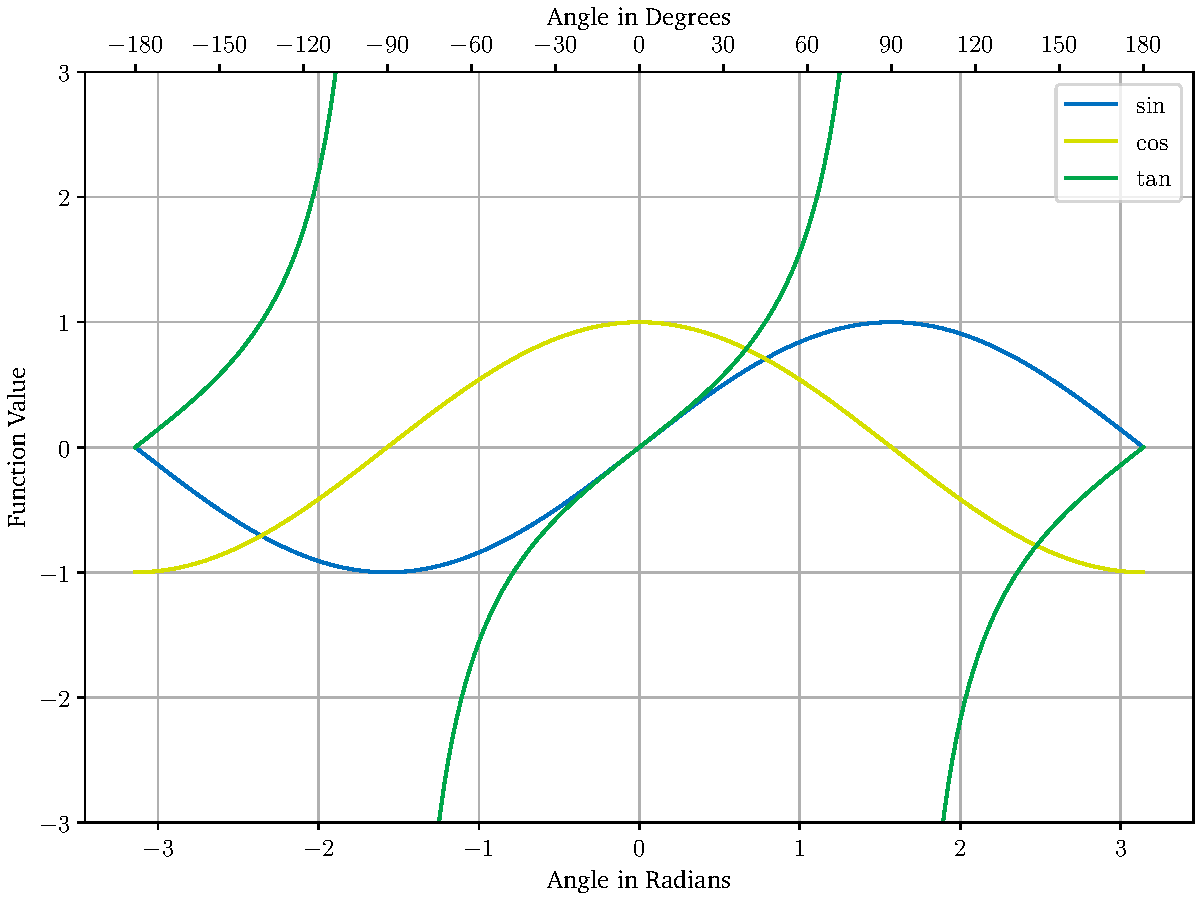
\includegraphics[width=\linewidth]{plots/trigonometric_functions.pdf}
    \caption[Plot comparison of trigonometric functions]{Plot comparison of trigonometric functions}
    \label{fig:trigonometric-func}
\end{figure}

Trigonometric functions are used as relation between apparent power $S$, active $P$ and reactive power $Q$.
While in discription of dynamics, the planning of networks or connection of machines, often the cosinodal function and therefore its value is present in the feeling of (engineering) people.
In stability analysis often the $\tan$ function is used, simply because its directly connecting onle active and reactive power, and because some athematic reformulations are possible with that. 
\autoref{fig:trigonometric-func} is illustrating relations of these functional values to the angle in rad and degree, while \autoref{tab:trigonometric-func} gives a numerical connection.
This shall increase the feeling and evaluation of this thesis readers.

\begin{table}[H]
    \centering
    \small
    \caption{Comparison of trigonometric functions dependent on the angle $\phi$ in degree or radians}
    \label{tab:trigonometric-func}
    \vspace*{12pt}
    \begin{tabularx}{\linewidth}{XXXXX}
        \textbf{Angle in $^\circ$} & \textbf{Angle in rad} & \textbf{$\sin$} & \textbf{$\cos$} & \textbf{$\tan$} \\ \toprule
        0   & 0         & 0         & 1         & 0 \\
        10  & 0.1745    & 0.1736    & 0.9848    & 0.1763 \\
        20  & 0.3490    & 0.3420    & 0.9397    & 0.3640 \\
        30  & 0.5236    & 0.5       & 0.8660    & 0.5774 \\
        40  & 0.6981    & 0.6428    & 0.7660    & 0.8391 \\
        50  & 0.8727    & 0.7660    & 0.6428    & 1.1918 \\ 
        60  & 1.0472    & 0.8660    & 0.5       & 1.7321 \\
        70  & 1.2217    & 0.9397    & 0.3420    & 2.7475 \\
        80  & 1.3962    & 0.9848    & 0.1736    & 5.6713 \\
        90  & 1.5708    & 1         & 0         & $\nexists$ \\
        120 & 2.0944    & 0.8660    & -0.5      & -1.7321 \\
        150 & 2.6180    & 0.5       & -0.8660   & -0.5774 \\
        180 & 3.1416    & 0         & -1        & 0 \\
        \bottomrule
    \end{tabularx}
\end{table}

\section{Description of the Power System Simulation process}
\label{app:power-system-modeling}

In this appendix section, the general process of power system simulation is described. As this thesis is aiming to understand voltage stability and processes in longer periods of time, these explanations apply to pointer-based simulations, called RMS simulations. Meaning that the considered effects are slower electromechanical nature instead of faster electromagnetic ones. The in this thesis used Python framework \glqq \textit{diffpssi}\grqq~is based on this type of simulation, and due to its open-source based nature traceable.

\begin{figure}[H]
    \centering
    % \includegraphics[width=\textwidth]{fundamentals/power-system-simulation-process.pdf}
    \missingfigure{Power system simulation process}
    \caption{Power system simulation process; own illustration}
    \label{fig:power-system-simulation-process}
\end{figure}

\commenting{
    Really basic: (?)
    \begin{itemize}
        \item RMS vs EMT simulation (-> meaning one cannot simulate other faults than 3ph w/o ground)
        \item Phasor description
        \item Basic formulation: Static (algebraic) and dynamic (differential) equations
        \item Using of solvers (Integrators) for time domain simulation
        \item Using of different optimizatinon algorithms for steady state (load flow) simulation -> initial values
    \end{itemize}
    Less basic and more advanced:
    \begin{itemize}
        \item rountines in the framework
        \item two types: Algebraic and Differential equations have to be solved at each time step -> What is which? Which operational equipment is typically described with which type of equation?
        \item per unit system applying for easier simulation (different voltage levels)
        \item ...
    \end{itemize}
}

%%%%%%%%%%%%%%%%%%%%%%%%%%%%%%%%%%%%%%%%%%
% \section{Jacobian based voltage stability criterions}
% \label{app:jacobian-voltage-indices}

% \textcite{danish_2015} is showing, describing, and referencing some voltage stability indices based on the Jacobian matrix. The following table is a collection of these indices.

% \begin{sidewaystable}[H]
%     \centering
%     \small
%     \caption{Jacobian based voltage stability criterions; after \textcite{danish_2015}}
%     \vspace*{12pt}
%     \renewcommand{\arraystretch}{2}
%     \begin{tabularx}{23cm}{llXXl}
%         % \toprule
%         \textbf{Index} & \textbf{Abbreviation} & \textbf{Calculation} & \textbf{Stability Threshold} & \textbf{Reference} \\
%         \toprule
%         Tangent Vector Index & \acs{TVI} & $\mathrm{TVI}_i=\left\lvert \frac{\dd{V_i}}{\dd{\lambda}}\right\rvert^{-1}$ & depending on load increase & \\ \midrule
%         Test Function & & $t_{cc}=\left\lvert e^T_c \cdot \mab{J} \times \mab{J}_{cc}^{-1} \cdot e_c\right\rvert$ & details are given in reference & \\ \midrule
%         Second Order Index & $i$ & $i=\frac{1}{i_0} \cdot \sigma_\mathrm{max} \cdot \big( \dv{\sigma_\mathrm{max}}{\lambda_\mathrm{total}} \big)^{-1}$ & $i > 0$ & \\ \midrule
%         Minimum Eigenvalue & & $\Delta V=\sum_{i} \frac{\xi_i\eta_i}{\lambda_i} \Delta Q$ & all eigenvalues should be positive & \\ \midrule
%         Minimum Singular Value & & $\begin{bmatrix} \Delta \vartheta \\ \Delta V \end{bmatrix}=\mab{V} \sum^-1 \mab{U}^T \begin{bmatrix} \Delta F \\ \Delta G \end{bmatrix}$ & details are given in reference & \\ \midrule
%         Predicting Voltage Collapse & & $\frac{V}{V_0}$ & the smallest index value & \\ \midrule
%         Impedance Ratio & & $\frac{Z_ii}{Z_i}$ & $\frac{Z_ii}{Z_i} \leq 1$ & \\
%         \bottomrule
%     \end{tabularx}
% \end{sidewaystable}



% %%%%%%%%%%%%%%%%%%%%%%%%%%%%%%%%%%%%%%%%%%
% \section{Comparison of System based and Jacobian based indices}
% \label{app:jacobian-vs-system-indices}

% %%%%%%%%%%%%%%%%%%%%%%%%%%%%%%%%%%%%%%%%%%
% %%%%%%%%%%%%%%%%%%%%%%%%%%%%%%%%%%%%%%%%%%
\chapter{Modeling}

%%%%%%%%%%%%%%%%%%%%%%%%%%%%%%%%%%%%%%%%%%
\section{Admittance Calculation of a Two-Port}
\label{app:admittance-deduction}

Follwing part shall just give a short, but complete and clear overview, how the admittance matrix of a two-port system is calculated.
Therefore the main focus of this thesis, a two-port with variable translation ratio, is kept.

%%%%%%%%%%%%%%%%%%%%%%%%%%%%%%%%%%%%%%%%%%
\section{Analytical Calculation of Simple Nose Curves}
\label{app:analytical-nose-curve}

Some blibla and equations about the analytical calculation of simple nose curves.


%%%%%%%%%%%%%%%%%%%%%%%%%%%%%%%%%%%%%%%%%%
\section{Alternative Current Injection Model}
\label{app:current-injection-model}

\textcite{machowski_2020} describes another way of modeling a \acs{OLTC} transformer with variable ratio.
This model is looking at the shunt brnaches as current injections, which are added to the individual busses.
Beneficial, the system admittance matrix is staying symmetrical, while the different transformer state(s) are represented by the different current injections.
This can be mathematically expressed by following set of equations:
\begin{align}
    \begin{bmatrix}
        \underline{I}_1 \\
        -\underline{I}_2
    \end{bmatrix} &=
    \begin{bmatrix}
        \underline{Y}_\mathrm{T} & -\underline{Y}_\mathrm{T} \\
        -\underline{Y}_\mathrm{T} & \underline{Y}_\mathrm{T}
    \end{bmatrix}
    \begin{bmatrix}
        \underline{U}_1 \\
        \underline{U}_2
    \end{bmatrix} -
    \begin{bmatrix}
        \Delta \underline{I}_1 \\
        \Delta \underline{I}_2
    \end{bmatrix}\text{, where } \notag \\[12pt]
    \begin{bmatrix}
        \Delta \underline{I}_1 \\
        \Delta \underline{I}_2
    \end{bmatrix} &=
    \begin{bmatrix}
        \underline{0} & (\underline{\vartheta}-1)\underline{Y}_\mathrm{T} \\
        -(\underline{\vartheta}^*+1)\underline{Y}_\mathrm{T} & (\underline{\vartheta}^*\underline{\vartheta}+1)\underline{Y}_\mathrm{T}
    \end{bmatrix}
    \begin{bmatrix}
        \underline{U}_1 \\
        \underline{U}_2
    \end{bmatrix} \text{ leading to } \notag \\[12pt]
    \underline{\mab{Y}}_\mathrm{\Pi,T,Current~Injection}&= 
    \begin{bmatrix}
        \underline{Y}_\mathrm{T} & -\underline{Y}_\mathrm{T} \\
        -\underline{Y}_\mathrm{T} & \underline{Y}_\mathrm{T}
    \end{bmatrix} -
    \begin{bmatrix}
        \underline{0} & (\underline{\vartheta}-1)\underline{Y}_\mathrm{T} \\
        -(\underline{\vartheta}^*+1)\underline{Y}_\mathrm{T} & (\underline{\vartheta}^*\underline{\vartheta}+1)\underline{Y}_\mathrm{T}
    \end{bmatrix} \notag % \label{eq:admittance-oltc-2}
\end{align}

%%%%%%%%%%%%%%%%%%%%%%%%%%%%%%%%%%%%%%%%%%
\section{Program Structure for the discrete OLTC Control}

\begin{figure}[H]
    \centering
    \missingfigure{Program Plan OLTC}
    \caption[Program or algorithmic structure for the control scheme of the OLTC control]{Program or algorithmic structure for the control scheme of the OLTC control}
    \label{fig:oltc-program-plan}
\end{figure}

%%%%%%%%%%%%%%%%%%%%%%%%%%%%%%%%%%%%%%%%%%
\section{Program Structure for the discrete FSM Control}

\begin{figure}[H]
    \centering
    \missingfigure{Program Plan FSM}
    \caption[Program or algorithmic structure for the control scheme of the FSM control]{Program or algorithmic structure for the control scheme of the FSM control}
    \label{fig:fsm-program-plan}
\end{figure}

%%%%%%%%%%%%%%%%%%%%%%%%%%%%%%%%%%%%%%%%%%
\section{Class Diagrams}

\subsection{Extended Class Diagram of the Transformer Architecture}

\subsection{Extended Class Diagram of the OLTC Transformer}

\subsection{Extended Class Diagram of the Discrete OLTC Control}
\subsection{Extended Class Diagram of the Discrete FSM Control}

\subsection{Class Diagram of the Class Nose Curves}
\label{app:nose-curve}

\begin{figure}[H]
    \centering
    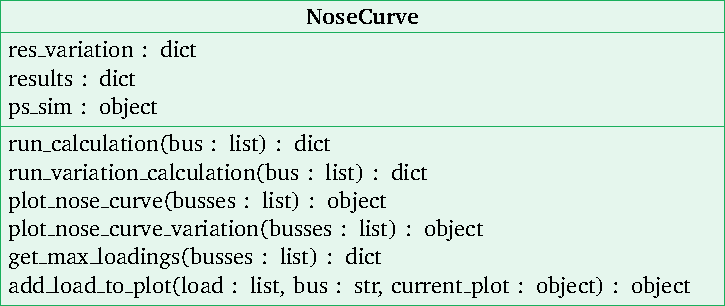
\includegraphics[width=12cm]{tikz_graphics/images/class_diagram_nosecurve_complete.pdf}
    \caption{Complete class diagram of the class Nose Curves; including all attributes and methods with data types, returns, and inputs}
    \label{fig:class-diagram-nose-curves}
\end{figure}


\subsection{Extended Class Diagram of the Class ViolationIntegral}
\subsection{Extended Class Diagram of the Class CriticalTimes}

% %%%%%%%%%%%%%%%%%%%%%%%%%%%%%%%%%%%%%%%%%%
% \section{OLTC control}


%%%%%%%%%%%%%%%%%%%%%%%%%%%%%%%%%%%%%%%%%%
%%%%%%%%%%%%%%%%%%%%%%%%%%%%%%%%%%%%%%%%%%
\chapter{Validation}
\label{app:validation}

%%%%%%%%%%%%%%%%%%%%%%%%%%%%%%%%%%%%%%%%%%
\section{Datails About Used Networks}
\label{app:networks}

\subsection{Single-Machine Infinite Bus-Bar Model}
\label{app:smib-model}

\commenting{Table with parameter details}

\subsection{SMIB Model with Additional Load}
\label{app:smib-w-load}

\commenting{Table with parameter details}


%%%%%%%%%%%%%%%%%%%%%%%%%%%%%%%%%%%%%%%%%%
\section{Additional Plots from the  Pi Model Validation}
\label{app:add-validation-plots}

\begin{figure}[H]
    \centering
    \includegraphics[width=\linewidth]{development_files/validation/data/s_n_comp_complete.pdf}
    \caption[Model results concerning the variation of the rated apparent power]{Voltage results of the $\Pi$-modeled transformer in the \acs{SMIB} model between PowerFactory and the Python framework; Variation of the rated apparent power $S_\mathrm{n}$; Left column is showing the data for the Pathon module \textit{diffpssi}, on the right the comparative tool \textit{DIgSILENT PowerFactory}}
    \label{fig:valid-s-compl}
\end{figure}

\begin{figure}[H]
    \centering
    \includegraphics[width=\linewidth]{development_files/validation/data/s_n_comp_1100mva.pdf}
    \caption{Comparison of one variation parameter between \textit{diffpssi} and \textit{DIgSILENT PowerFactory}; each plot focussing on one bus in the variation of the rated apparent power $S_\mathrm{n}$}
    \label{fig:valid-s-1100}
\end{figure}

\begin{figure}[H]
    \centering
    \includegraphics[width=\linewidth]{development_files/validation/data/theta_comp_complete.pdf}
    \caption{Comparison of the $\Pi$-modeled transformer in the \acs{SMIB} model between PowerFactory and the Python framework}
    \label{fig:valid-ratio-comp}
\end{figure}

\begin{figure}[H]
    \centering
    \includegraphics[width=\linewidth]{development_files/validation/data/theta_comp_ratio09.pdf}
    \caption{Comparison of one variation parameter between \textit{diffpssi} and \textit{DIgSILENT PowerFactory}; each plot focussing on one bus in the variation of the longitudinal transformer ratio $\vartheta$}
    \label{fig:valid-ratio-09}
\end{figure}

%%%%%%%%%%%%%%%%%%%%%%%%%%%%%%%%%%%%%%%%%%
\section{Additional Plots from the Tap Changer Control Schemes}
\label{app:add-validation-tap-changer}

\subsection{OLTC validation}

For simple load:
\begin{figure}[H]
    \centering
    \includegraphics[width=\linewidth]{development_files/validation/data/tds_oltc_simple-load.pdf}
    \caption{\acf{TDS} for standard discrete \acs{OLTC} control scheme applied to the simple load network}
    \label{fig:valid-ratio-09}
\end{figure}

For SMIB with load:
\begin{figure}[H]
    \centering
    \includegraphics[width=\linewidth]{development_files/validation/data/tds_oltc_ex-smib.pdf}
    \caption[Time Domain Result of the OLTC control scheme applied on the extended \acs{SMIB} network]{\acf{TDS} of the standard discrete \acs{OLTC} control scheme; Result of the extended or modified \acs{SMIB} model with additional load}
    \label{fig:tds-oltc-ex-smib}
\end{figure}

\begin{figure}[H]
    \centering
    \includegraphics[width=\linewidth]{development_files/validation/data/oltc_ex-smib_integrator.pdf}
    \caption{Internal signal of the standard discrete \acs{OLTC} control: The integrator signal, representing the time constant for enabling the switching operation}
    \label{fig:int-signal-oltc-ext-smib-integrator}
\end{figure}

\subsection{FSM validation}

For simple load:
\begin{figure}[H]
    \centering
    \includegraphics[width=\linewidth]{development_files/validation/data/signal_vdead_fsm_simple.pdf}
    \caption{Signal evolution for the voltage difference dependent \acs{FSM} control scheme; Plot of the deadband filtered voltage difference $v_\mathrm{dead}$ for the simple load validation case}
    \label{fig:signal-vdead-fsm-simple}
\end{figure}

For SMIB with load:

\begin{figure}[H]
    \centering
    \includegraphics[width=\linewidth]{development_files/validation/data/tds_fsm_vdiff.pdf}
    \caption[\acs{TDS} for a \acs{FSM} control scheme switching based on the voltage difference]{\acs{TDS} for a \acs{FSM} control scheme switching based on the voltage difference}
    \label{fig:tds-fsm-vdiff-ext-smib}
\end{figure}


\begin{figure}[H]
    \centering
    \includegraphics[width=\linewidth]{development_files/validation/data/tds_fsm_preferred.pdf}
    \caption[Differing \acs{TDS} for a \acs{FSM} control scheme preferring the \acs{FSM}]{Differing \acs{TDS} for a \acs{FSM} control scheme preferring the \acs{FSM}}
    \label{fig:tds-fsm-preferred}
\end{figure}

%%%%%%%%%%%%%%%%%%%%%%%%%%%%%%%%%%%%%%%%%%
%%%%%%%%%%%%%%%%%%%%%%%%%%%%%%%%%%%%%%%%%%
\chapter{Case study}

\end{document}
%------------------------- Ende des Dokuments -----------------------